\chapter{Vision-Based Control of Humanoid Walking} 
\label{Chap:Visual-Servoing}

We have introduced the mathematical foundations behind humanoid walking. In this chapter we will discuss the applicability of controlling the robot trajectory using visual servoing, as depicted in Fig.~\ref{Fig:Schema}. We present a novel approach for using a visual servoing scheme to control the dynamic walk of a humanoid robot. Here, the online information given by an on-board camera is used to drive the robot towards a specific goal, in a visual servoing scheme. This closed loop approach allows the system to react to changes in its environment and to adapt to modeling errors. Our work is built upon the reactive pattern generator of \citep{HerdtAR2010} that we presented at the end of Chapter \ref{Chap:Locomotion-Control}, which modifies footsteps, center of mass and center of pressure trajectories to track a reference velocity. We compare our method to another which does not use Model Predictive Control in the visual servoing. This alternative method, proposed by Dune et al. \citep{DuneIROS2010} outputs, in a first stage, a reference velocity directly given by the visual servoing control law and then, in a second stage, this reference velocity is introduced in the pattern generator to produce the appropriate walking motion (hence, our term of ``decoupled''). The coupled approach proposed here uses a Model Predictive Control scheme to introduce the visual error terms directly within the pattern generator. This allows to avoid a number of limitations (e.g. that visual constraints cannot be introduced directly inside the locomotion controller or that the camera motion has to be accounted separately) that appear in the decoupled method.  In this work, both approaches are compared numerically and validated in simulation.

\section{ Visual servoing}

Visual servoing aims at controlling the motion of a robot equipped with a camera, by minimizing errors between observed features and their corresponding reference features, \citep{ChaumetteRAM2006, ChaumetteRAM2007}. The nature of the features differentiates schemes of visual servoing: Image based visual servoing (IBVS) uses only image features; Position based visual servoing (PBVS) uses the 3-D pose(s) of object(s) of interest. In any of these cases of feedback, one may use a velocity controller such as

$$
\text{v}^c = -\lambda {L}_e^{+} {e},
$$

\noindent where ${e} = {s}-{s}^{*}$ is the vector of errors between the current features $s$ and the desired ones ${s}^{*}$, $\text{{v}}^c$ is the velocity of the camera (the control variable), and ${L}_e^{+}$ is the Moore-Penrose pseudo-inverse of the interaction matrix ${L}_e$, that is, the matrix relating the velocity of the features and the velocity of the camera.

\begin{figure}[ht] 
\begin{center}
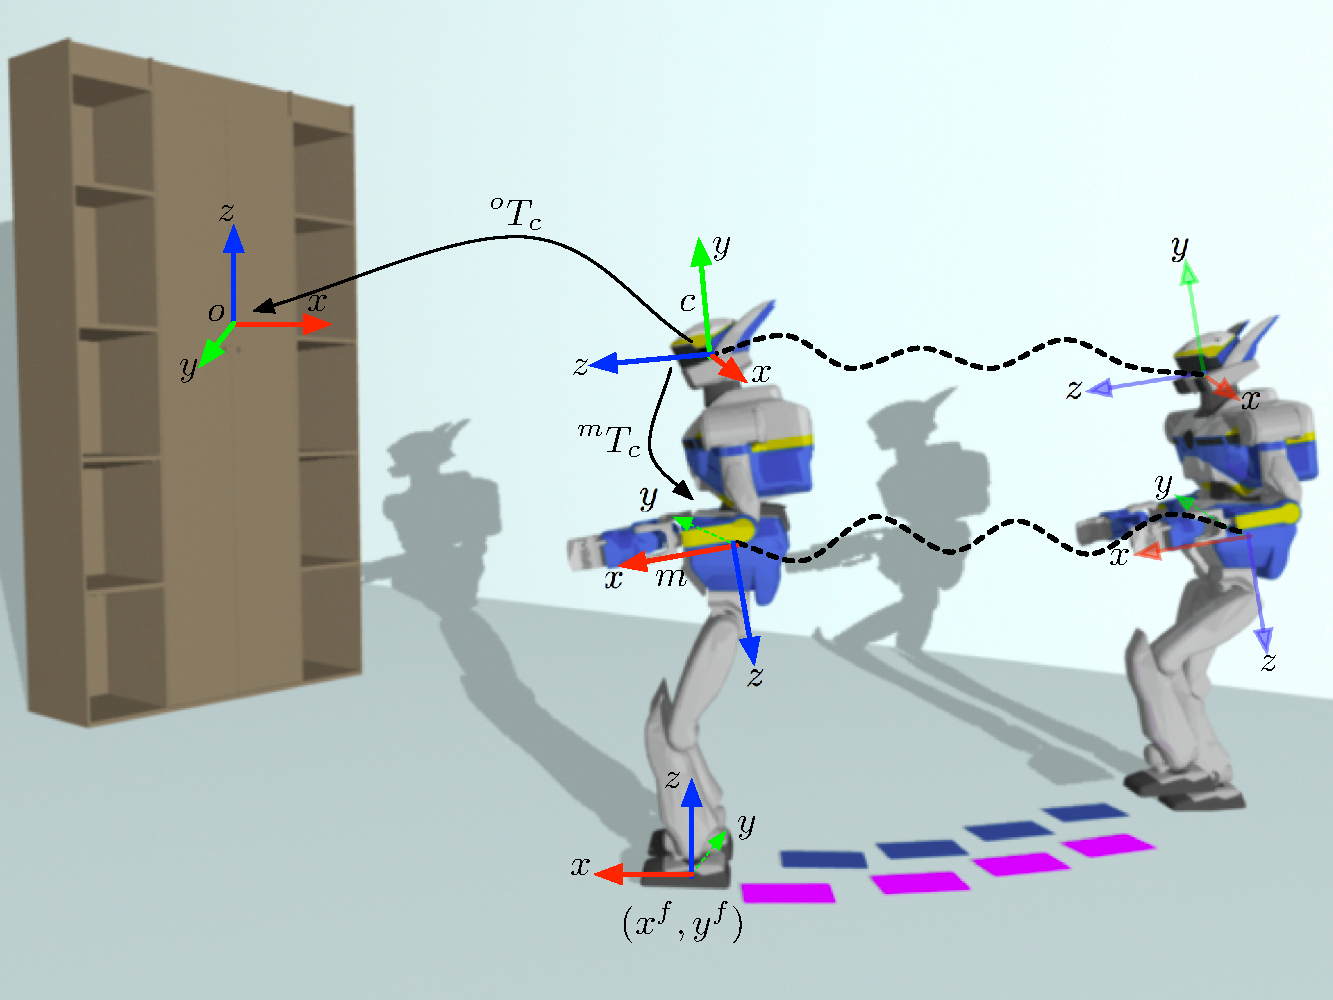
\includegraphics[scale=0.5]{Chap4-Visual-Servoing/schema_new.pdf} 
\caption{ An example setup for our approach: the robot has to walk towards a desired position with regards to an object viewpoint. Frames $o$, $c$ and $m$ refer to the {\it object}, {\it camera} and {\it CoM} respectively. $^o {T}_c$ is the transformation to view the camera points in the object reference frame. $(x^f, y^f)$ is the current footprint position.} 
\label{Fig:Schema}
\end{center}
\end{figure}

We will now describe two approaches for introducing visual control in the described pattern generation: the first one (in Section~\ref{sec:vsclaire}) is a decoupled one, proposed by Dune et al. \citep{DuneIROS2010}, where the visual servoing is used to determine the reference velocity in Eq.~\ref{Eq:MinJerk}; the second one (Section~\ref{sec:vsmauricio}) modifies Eq.~\ref{Eq:MinJerk} to replace the reference velocity term by a new term directly related to the decreasing of the visual errors.


\section{Visual Control Using a Reference Velocity}
\label{sec:vsclaire}


As for any pattern generator, the stepping motion induces a sway motion, which can be read as the difference existing between the reference velocity used in the Eq.~\ref{Eq:MinJerk} of the Model Predictive Control and the real velocity effectively attained from the first control. This sway motion is necessary for a proper walk, but it obviously generates non-desired effects on the robot visual perception. As stated in~\citep{DuneIROS2010}, the result of this sway motion on the real camera velocity $\text{v}^c$ can be modeled as:

\begin{equation}
\text{{v}}^c =\overline{\text{{v}}}^c+{^{c}  V_{m}} \text{{v}}^b
\label{eq:sway}
\end{equation}

\noindent where $\overline{\text{{v}}}^c$ is the ``ideal'' camera velocity that would exist without sway, and $\text{{v}}^b$ is the part of the CoM velocity that is induced by the sway. The matrix ${^c  V_{m}}$ is a $6\times6$ twist matrix relating the camera frame (index ``c'') to the CoM frame (index ``m'') through the transform ${^cT_{m}}$.

We recall how in~\citep{DuneIROS2010}, a classical visual servoing scheme is adapted to be used for a humanoid robot. The idea, basically, is to use the output velocity from Eq.~\ref{eq:avControlCom} as a reference velocity for Eq.~\ref{Eq:MinJerk}. However, as we have pointed it out, the humanoid motion has an intrinsic sway component, that makes the visual features have an evolution in the image not corresponding to the desired trajectory. 

As mentioned above, the features motion in the image can be decomposed into a component due to the sway motion, and a component due to the ``average'' (sway-less) motion of the robot,

\begin{equation}
\label{Eq:FeaturesSway}
\dot{ s}={ L_e} \overline{\text{v}}^c+ { L_e} \, ^c  V_{m}{\text{v}^{b}}.
\end{equation}

Then, the idea is to use a virtual camera that would correspond to the position of the camera if we supposed that there were no sway motion affecting the robot motion, to control this virtual camera, and use its controlled velocity ($\overline{\text{ v}}^c$) as a reference velocity in the reactive PG.
 
%----------------------FIG-----------------------------------------------%
%\begin{figure}[ht] 
%\begin{center}
%\includegraphics[width=\columnwidth]{images/correction.ps} 
%\vspace{-1cm} 
%\caption{ $\Rep{K}$ is the current camera frame and $\overline{\Rep{K}}$ is the camera position obtained if the visual servoing velocity is applied without the walking constraints.} 
%\label{fig:frames}

%\end{center}
%\vspace{-0.5cm} 
%\end{figure}
%------------------------------------------------------------------------%

Integrating equation \ref{Eq:FeaturesSway} between $0$ and $t$, Dune et al. have shown that the relationship between the real observed features $s(t)$ and the ``sway-less'' features $\bar{s}(t)$ can be written as

\begin{equation}
s(t) = \overline{s}(t) + \int_{0}^{t} {{\widehat{ L_e}}} \, ^c  V_{m} \text{ v}^b dt - E,
\end{equation}

\noindent where $E \stackrel{\mbox{\tiny def}}{=} s(0)-\overline{s}(0)$. From the previous equation, the corrected visual error between a reference features vector and the sway-less features vector, to be used for the computation of the reference velocity, is deduced as

\begin{align}
\overline{e}(t)&=\overline{s}(t) -s^*= e(t) -  (\int_{0}^{t}{ {\widehat{ L_e}}} \, ^c  V_m \text{ v}^b dt -E).
\end{align}

Under this model, the virtual error $\overline{e}(t)$ is regulated to zero, and the real error $e(t)$ is oscillating around zero, with a period $T$, because of the sway.

The shift $E$ is re-estimated regularly over one period of time (e.g., the last period) by 

$$
E= \frac{1}{T^{sway}}\int_{t-T^{sway}}^t\int_0^t { {\widehat{ L_e}}} \, ^c  V_m \text{ v}^b  dt dt,
$$ 

\noindent and finally, it is used in the control law for the CoM (e.g., the reference velocity for Eq.~\ref{Eq:MinJerk}) 

\begin{gather} 
\overline{\text{ v}}^m= -\lambda{ ^c  V_m {{ {\widehat{ L_e}}}}^{+}}(e -  (\int_{0}^{t}{{ {\widehat{ L_e}}}} \, ^c  V_{m}\text{ v}^b dt - E)).
\label{eq:avControlCom} 
\end{gather} 

Note that the discrete form of the involved integrals are used in practice. More details can be found in~\citep{DuneIROS2010}. To apply this control, we need the actual measured errors $ e$ (as in any classical visual servoing approach), an estimate of the sway motion period, which is deduced from the stepping period, and a point-wise estimate for the sway motion at the level of the CoM $\text{ v}^b$.

This reference velocity can be directly injected in the Velocity Controlled Pattern Generator introduced in previous section. However, this approach has several drawbacks. First, the control law will never be executed as is, because of dynamical and physical limitations of the robot. Second, to get equation \ref{eq:avControlCom}, they make several assumptions, which sometimes are not true. And third, since the PG and the servo controller are totally decoupled, the visual feedback has to wait for the next iteration to be introduced in the PG. In order to solve this problem, we will present in the next section a Visual Servo controller which will be directly introduced in the Pattern Generator.

\section{Visual servoing and MPC}
\label{sec:vsmauricio}

As we know, in walking pattern generation, MPC is used to estimate a sequence of optimal controls at some horizon, because of the step-based nature of walking. Hence, we want to orient the optimization of the foot placement by taking into account the expected evolution of the visual servoing (VS) errors so that, instead of minimizing the VS errors at current time $k$, one would like to foresee its evolution at some horizon $[k+1,k+N]$. In this chapter, in order to simplify the notation, we will use the form $s_k$ to express the time reference $k$ of $s(k)$ and alike.

In~\citep{Allibert2010}, such a time horizon-aware scheme has been proposed. The visual predictive control (VPC) is introduced as:

\begin{eqnarray}
\label{Eq:MinVisualFeatures}
 \min_{U_{k}} \;&& \sum\limits_{j=k+1}^{k+N} [ s^d_j - s^m_j]^{\transpose} W_j [s^d_j - s^m_j], \\
 \mbox{subject to} \; && s^d_j = s^{*}_j - \epsilon_j, \\
 \label{Eq:ConstraintDynamicModel}
 && q_j = f(q_{j-1},u_{j-1}), \\
 \label{Eq:ConstraintProjection}
 && s^m_j = h(q_j).
\end{eqnarray}

In Eq.~\ref{Eq:MinVisualFeatures}, $U_{k}=u_{k:k+N-1}$ are the series of controls to be applied, $q_j$ is the state, and $s^*_j$, $s^d_j$ and $s^m_j$ are respectively the reference, desired and predicted positions of the visual features. The terms $\epsilon_j$ are the errors $s_j-s^m_j$ between real and predicted feature positions.
Allibert et al. assume $\epsilon_j$ constant over the prediction horizon, equal to $\epsilon_k=s_k-s^m_k$, i.e. the error at current time $k$, because by definition the $s_j$ are not known for $j>k$.
Since our landmarks are static, $s^*_j \stackrel{\mbox{\tiny def}}{=} s^*$, and since the prediction errors are constant on the horizon window, $s^d_j=s^d_k=s^*-\epsilon_k$ are constant in the prediction horizon.

Eq.~\ref{Eq:ConstraintDynamicModel} is the dynamic model, that estimates the new state given the last state/control pair. In general, this function is non-linear. We will see how to deal with this non-linearity.

Eq.~\ref{Eq:ConstraintProjection} is also a non-linear function that estimates the output of the model $s^m_j$, given the current state $q_j$. This equation implements the pinhole camera projection model.

Matrix $W_j$ in Eq.~\ref{Eq:MinVisualFeatures} is a positive definite matrix  used to weight errors in the prediction horizon. As suggested in~\citep{Allibert2010}, we   consider equal weights for all features errors, $W_j = diag(w_j)$. 

Here, $s^m_j$ is the collection of all the predicted features at time $j$, that is, for $M$ features $s^m_j = ( s_{1,j}^m, s_{2,j}^m, \hdots, s_{M,j}^m )^{\transpose} $. Eq.~\ref{Eq:MinVisualFeatures} can be rewritten as

\begin{equation}
\label{Eq:MinVisualFeatures2}
 \min_{U_{k}} \; \sum\limits_{l=0}^{M}  [S^d_{l} - S^m_{l,k}]^{\transpose} W [S^d_{l} - S^m_{l,k}],
\end{equation}

\noindent with $S^m_{l,k} =  \left(
  s^m_{l,k+1},
  s^m_{l,k+2},
 \dots,
  s^m_{l,k+N}
 \right)^{\transpose}$ stacking the features positions in the horizon, $S^d_{l}$ stacking the corresponding desired positions, and the weights matrix $W = diag(w_{k+1},w_{k+2},...,w_{k+N})$.

Allibert et al. solved directly the non-linear programming problem Eqs.~\ref{Eq:MinVisualFeatures}-\ref{Eq:ConstraintProjection} to compute the controls in their visual servoing scheme.

\section{Integrating the visual servoing to the walking motion generator}
\label{sec:integration}
In the following we use superscripts $w,c,m$ to refer the world, the camera, and the CoM reference frame, and ${^cT_{m}}$ means transformation from $c$ to $m$ frame. If we introduce directly Eq. \ref{Eq:MinVisualFeatures2} in Eq. \ref{Eq:MinJerk}, we will not have a QP anymore due to the non-linear constraints, namely Eqs. \ref{Eq:ConstraintDynamicModel} and \ref{Eq:ConstraintProjection}. We can directly solve the first problem (Eq. \ref{Eq:ConstraintDynamicModel}) by using the dynamic model in Eq. \ref{Eq:PosCMHorizon}. In this case there is no rotation, but we will see that we can introduce it in a decoupled way without losing the QP formulation.

\subsection{Linearization of the observation model}

As we said, Eq. \ref{Eq:ConstraintProjection} implements the pinhole camera model. Let $^{w}p_{l'} = [^{w}x_{l'},^{w}y_{l'},^{w}z_{l'}]^{\transpose}$ be the position of the {l'}-th landmark in the world reference frame. At time $j$, one can compute the projection to the image plane by first transforming the landmark position to the camera frame with the homogeneous transform $^mT_c {^wT_{m,j}}$ and then applying the projection,

\begin{equation}
\label{Eq:Projection}
\begin{array}{c}
 \left(
 \begin{matrix}
  u_{l',j} \\
  v_{l',j}
\end{matrix}
\right)
  =
 \left(
 \begin{matrix}
  u({^cx_{l',j}},{^cy_{l',j}},{^cz_{l',j}}) \\
  v({^cx_{l',j}},{^cy_{l',j}},{^cz_{l',j}})
 \end{matrix}
 \right)
 =  \left(
 \begin{matrix}
  {^cx_{l',j}} / {^cz_{l',j}}\\
  {^cy_{l',j}} / {^cz_{l',j}}
 \end{matrix}
 \right),
 \end{array}
\end{equation}

\noindent where $^wT_{m,j}$ is the transformation from the world frame to the CoM frame at time $j$ and $^mT_c$ is the transformation from the CoM frame to the camera frame, which is not variable in our approach. Note that

$$
^wT_{m,j} = (^mT_{w,j})^{-1} = 
\left(
\begin{matrix}
(^mR_{w,j})^{-1} & -(^mR_{w,j})^{-1} {^mt_{w,j}}\\
0_{1 \times 3} & 1
\end{matrix}
\right)
$$ 

\noindent where $^mt_{w,j}$ is the position of the CoM in the world frame at time $j$, which depends in our control variables through Eq. \ref{Eq:PosCMHorizon}.
$^mR_{w,j}$ is the direction of the robot waist according to the world reference frame at time $j$. In our current formulation 
there is no free variables modifying this quantity, because it would make the problem non-linear. More details
about this problem are given in Section~\ref{subsection:control_of_the_rotation_angle}.

If we use directly Eq. \ref{Eq:Projection} (non-linear), we will lose the QP formulation. 
We know that Eq.~\ref{Eq:Projection} is a projection $h:\mathbb{R}^3 \rightarrow \mathbb{R}^2$.

\begin{equation*}
%\label{Eq:ProjectionTaylor}
h(x,y,z) =
 \left(
 \begin{matrix}
  u(x,y,z) \\
  v(x,y,z)
 \end{matrix}
 \right)
 = \left(
 \begin{matrix}
  x / z\\
  y / z
 \end{matrix}
 \right).
\end{equation*}


We also know from MPC that prediction is done over a finite horizon. So it might be enough to use a first order approximation of $h$ for small $(dx,dy,dz)$ so that we can maintain the QP form.

Now, by using a Taylor series for $u(x,y,z)$ around some point $(x_0,y_0,z_0)$ and substituting the derivatives,

%$$
%\begin{array}{c}
% u(x_0+dx,y_0+dy,z_0+dz) = u(x_0,y_0,z_0) +\\
% u_x(x_0,y_0,z_0)dx + u_y(x_0,y_0,z_0)dy + \\
% u_z(x_0,y_0,z_0)dz + \mathcal{O}(dx,dy,dz)^2
%\end{array}
%$$

$$
\left\{
\begin{array}{c}
%\label{Eq:ProjectionTaylorApproxU}
\nonumber
 u(x_0+dx,y_0+dy,z_0+dz) \approx \dfrac{x_0}{z_0} +  \dfrac{dx}{z_0} - \dfrac{x_0 dz}{z_0^2},\\ \\
 v(x_0+dx,y_0+dy,z_0+dz) \approx \dfrac{y_0}{z_0} +  \dfrac{dy}{z_0} - \dfrac{y_0 dz}{z_0^2}.
\end{array}
\right.
$$

\noindent with $dx=x-x_0$, $dy=y-y_0$ and $dz=z-z_0$. 

We propose to apply such a linearization of Eq.~\ref{Eq:Projection} for the whole horizon, around the first position $(j=k)$ of landmark $l'$, i.e. at the linearization point $(^{c}x_{l',k},^{c}y_{l',k},^{c}z_{l',k})$, that is, the point we are actually watching in the CoM frame. 

This way, we can express the predicted position of the landmark $l'$ linearly at time $j>k$ in the horizon:

\begin{equation*}
%\label{Eq:ProjectionLinearized}
 \left(
 \begin{matrix}
  u_{l',j} \\
  v_{l',j}
 \end{matrix}
 \right)
 = \left(
 \begin{matrix}
  \pi^{11}_{l',k} \ ^{c}x_{l',j} + \pi^{13}_{l',k} \ ^{c}z_{l',j}+ u_{l',k}\\
  \pi^{22}_{l',k} \ ^{c}y_{l',j} + \pi^{23}_{l',k} \ ^{c}z_{l',j} + v_{l',k}
 \end{matrix}
 \right),
\end{equation*}

\noindent where $u_{l',k} = {^cx_{l',k}} / {^cz_{l',k}}$ and $v_{l',k} = {^cy_{l',k}} / {^cz_{l',k}}$ are the initial image positions of the landmarks in the horizon and the coefficients $\pi^{ij}_{l',k}$ the elements of the matrix

\begin{equation*}
\Pi_{l',k} = \left(
\begin{matrix}
 1/^{c}z_{l',k} & 0 & - u_{l',k} / ^{c}z_{l',k} \\
 0 & 1/^{c}z_{l',k} & - v_{l',k} / ^{c}z_{l',k}
\end{matrix}
\right),
\end{equation*}

\noindent which is the classical definition of the interaction matrix in Image-Based Visual Servoing.

Finally, we can express the projection of the $l'-th$ landmark (constraint \ref{Eq:ConstraintProjection}) as:

\begin{equation}
\label{Eq:Features}
 \left(
 \begin{matrix}
  u_{l',j} \\
  v_{l',j}
 \end{matrix}
 \right) = 
\left[
\begin{array}{cc}
\multirow{2}{*}{$\Pi_{l',k}$} & u_{l',k} \\
& v_{l',k} \\
\end{array}
\right]
 \ ^mT_c \ ^wT_{m,j} \left( \begin{array}{c}
 ^{w}p_{l'}\\
 1
 \end{array}\right),
\end{equation}

\noindent so that we can now introduce the visual features in the pattern generator. Expanding terms in Eq.~\ref{Eq:Features} for the first row and setting $\Pi^u_{l',k}$ as the first row of matrix $\Pi_{l',k}$,

\begin{eqnarray}
\label{Eq:FeatExpanded}
 u_{l',j} &= &\Pi^u_{l',k} (^wR_c {^wp_{l'}} + {^wR_c} {^mt_{w,j}} + {^mt_c}) + u_{l',k}.
\end{eqnarray}

Since $^wR_c {^mt_{w,j}} = {^wR_{c1}} x_j + {^wR_{c2}} y_j + {^wR_{c3}} z_j$, where $^wR_{ci}$ is the $i$-th column of $^wR_c$
\footnote{To simplify the notations ${^wR_c}={^mR_c}{^wR_{m,j}}$}
and $x_j,y_j,z_j$ the position of the CoM at time $j$ (see Chapter~\ref{Chap:Locomotion-Control}). We can rewrite Eq.~\ref{Eq:FeatExpanded}

\begin{equation}
\label{Eq:FeaturesUReduced}
 u_{l',j} = a^u_{l',k} x_j + b^u_{l',k} y_j + c^u_{l',k},
\end{equation}

\noindent with 
$$
\left\{
\begin{array}{ccl}
a^u_{l',k} & = & \Pi^u_{l',k} {^wR_{c1}}\\
b^u_{l',k} & = & \Pi^u_{l',k} {^wR_{c2}}\\
c^u_{l',k} & = & \Pi^u_{l',k} ({^wR_c} {^wp_{l'}} + {^mt_c} + {^wR_{c3}} z_j) + u_{l',k}.
\end{array}
\right.
$$
Equivalently,

\begin{equation}
\label{Eq:FeaturesVReduced}
  v_{l',j} = a^v_{l',k} x_j + b^v_{l',k} y_j + c^v_{l',k}.
\end{equation}

Stacking the features $u_{l',j}$ and the CoM positions for the whole horizon and using Eq.~\ref{Eq:PosCMHorizon}, we get a vector $S^m_{l,k}$ similar to the one introduced in Eq.~\ref{Eq:MinVisualFeatures2} 

\begin{equation*}
S^m_{l',k} = A^u_{l',k} C_x(k+1) + B^u_{l',k} C_y(k+1) + C_{l',k}^u,
\end{equation*}

\noindent with 
$$
\begin{array}{ccl}
A^u_{l',k} &=& a^u_{l',k} I_{N\times N}\\
B^u_{l',k} &=& b^u_{l',k} I_{N\times N}\\
C_{l',k}^u &=& c^u_{l',k} (1,1,...,1)^{\transpose}
\end{array}
$$

 \noindent which corresponds to the predicted coordinates $u$ of the landmark $l'$-th in the horizon.
The equivalent equations for the $v$ coordinates of the same landmark are straightforward.

Every projected landmark provides two coordinates $(u,v)$ and we treat each one as an individual feature. This means that the $l$-th feature is the $u$ coordinate in the image of the landmark $l' = \left \lfloor l/2 \right \rfloor$ for $l$ even, and the $v$ coordinate for $l$ odd.

Generalizing to all features, we have:
\begin{equation}
\label{Eq:FeaturesStacked}
 S^m_{l,k} = A_{l,k} C_x(k+1) + B_{l,k} C_y(k+1) + C_{l,k},
\end{equation}

\noindent with $A_{l,k} = A^u_{l',k}$ for $l$ even and $A_{l,k} = A^v_{l',k}$ for $l$ odd. The same holds for $B_{l,k}$ and $C_{l,k}$.

Finally, we can introduce visual servoing in the walking generation with the QP:

\begin{eqnarray*}
\label{Eq:MainQP}
\nonumber
 \min_{U(k)} \; && \dfrac{\alpha}{2} \left\| \dddot{C}_x(k) \right\|^2
 + \dfrac{\gamma}{2} \left\| Z_x(k+1) - Z_x^{ref}(k+1) \right\|^2 \\
 \nonumber
 && + \dfrac{\alpha}{2} \left\| \dddot{C}_y(k) \right\|^2
 + \dfrac{\gamma}{2} \left\| Z_y(k+1) - Z_y^{ref}(k+1) \right\|^2 \\
 \nonumber
 && + \dfrac{\beta}{2} \sum\limits_{l=0}^{M}  [S^d_{l}- S^m_{l,k}]^{\transpose} W [S^d_{l} - S^m_{l,k}],
\end{eqnarray*}

and as a canonical QP:
\begin{equation*}
\underset{U(k)}{\min} \; \dfrac{1}{2} U(k)^{\transpose} Q(k) U(k) + p(k)^{\transpose} U(k)
\end{equation*}

\text{ with }
\begin{equation*}
Q(k) = \left( \begin{array}{cc}
Q(k)' & 0 \\
0 & Q(k)'
\end{array}
 \right) + \hat{Q}(k),
\end{equation*}

\begin{equation*}
 Q(k)' = \left(
 \begin{array}{cc}
 \alpha I + \gamma U^{\transpose}_{z}U_{z} & - \gamma U^{\transpose}_{z}V \\
 -\gamma V^{\transpose} U_{z} & \gamma V^{\transpose} V
 \end{array}
 \right),
\end{equation*}

\begin{equation*}
 \hat{Q}(k) = \left(
 \begin{matrix}
 \beta \sum\limits_l U_{p}^{\transpose} A_{l,k}^{\transpose} {W} A_{l,k} U_{p} & 0 & \beta \sum\limits_l U_{p}^{\transpose} A_{l,k}^{\transpose} {W} B_{l,k} U_{p} & 0\\
 0 & 0 & 0 & 0 \\
 \beta \sum\limits_l U_{p}^{\transpose} B_{l,k}^{\transpose} {W} A_{l,k} U_{p} & 0 & \beta \sum\limits_l U_{p}^{\transpose} B_{l,k}^{\transpose} {W} B_{l,k} U_{p} & 0 \\
 0 & 0 & 0 & 0
 \end{matrix}
 \right)
\end{equation*}

and $p(k) = p(k)' + \hat{p}(k)$,

\begin{equation*}
 p'(k) = 
 \left(
 \begin{array}{c}
 \gamma U^{\transpose}_{z}(S_{z} \hat{c}_x(k) - V_c \hat{F}_x(k) \\
 -\gamma V^{\transpose}(S_{z}\hat{c}_x(k) - V_c \hat{F}_x(k) ) \\
 \gamma U^{\transpose}_{z}(S_{z} \hat{c}_y(k) - V_c \hat{F}_y(k) ) \\
 -\gamma V^{\transpose} (S_{z}\hat{c}_y(k) - V_c \hat{F}_y(k) )
 \end{array}
 \right),
\end{equation*}

\begin{equation*}
 \hat{p}(k) = 
 \left(
 \begin{matrix}
 \beta  \sum\limits_l U_{u}^{\transpose} A_{l,k}^{\transpose} W [A_{l,k} U_{s} \hat{c}_x(k) + B_{l,k} U_{s} \hat{c}_y(k) + C_{l,k} - S^d_l]\\
 0 \\
 \beta  \sum\limits_l U_{p}^{\transpose} B_{l,k}^{\transpose} W [A_{l,k} U_{s} \hat{c}_x(k) + B_{l,k} U_{s} \hat{c}_y(k) + C_{l,k} - S^d_l ]\\
 0
 \end{matrix}
 \right).
\end{equation*}

One must note in Eq.~\ref{Eq:MainQP}, unlike the velocity controlled PG, this QP does not include the reference velocity tracking, instead, it includes the minimization of the visual errors. It also includes the terms of the minimization of the jerks and the ZMP centering.

\subsection{Control of the rotation angle}
\label{subsection:control_of_the_rotation_angle}

So far, we have proposed a scheme to control the trajectory of the center of mass in the $xy$ plane. However, introducing the rotation angle in the minimization problem is not straightforward without losing linearity. Furthermore, the rotation angle plays a very important role here since sometimes most of the error between the desired features $s^d$ and the predicted features $s^m$ may be due to the angle between the robot and the features.

An extension of the original linear MPC scheme with automatic footstep placement that deals with a reference angular velocity has been proposed in~\citep{HerdtIROS2010}. The approach is a decoupled solution, that is, it estimates first the optimal rotation angles and afterwards introduces these values as known in the main QP (as the matrix ${^mR_{w,j}}$). This scheme should not affect the stability of the walking since inertial effects are not taken into account.

The same decoupled solution is used in this approach. Hence, in a first stage, we optimize the orientations in the MPC time window by  

{\small
\begin{eqnarray}
 \min\limits_{\dddot{C}_{\theta}(k),\dddot{F}_{\theta}(k) }  &&  \dfrac{\beta}{2} \left\| C_{\theta}(k+1) - \Theta^{0} \right\|^2 + \dfrac{\gamma}{2} \left\| F_{\theta}(k+1) - \Theta^{0} \right\|^2 \\
\nonumber && + \dfrac{\alpha}{2} \left\| \dddot{C}_{\theta}(k) \right\|^2 + \dfrac{\alpha}{2} \left\| \dddot{F}_{\theta}(k) \right\|^2,
\end{eqnarray}
}

\noindent with the same notations as for $\dddot{C}_x(k)$ and $\dddot{C}_y(k)$, $\dddot{C}_{\theta}(k)$ is the sequence of $N$ jerk values to be applied, and $C_{\theta}(k+1)$ is the sequence of predicted $\theta$ values, i.e. the orientations of the trunk,  

$$
C_{\theta}(k+1) \stackrel{\mbox{\tiny def}}{=} (c_{\theta}(k+1),...,c_{\theta}(k+N))^{\transpose},
$$

\noindent and similarly for $F_{\theta}(k+1)$, the feet orientations. Finally, as a reference orientation $\Theta^{0}$ is defined once for all at the starting configuration as a target feet orientation. Several conventions exist, in this paper, the trunk orientation $C_{\theta}(k)$ is trying to follow the flying foot orientation $F_{\theta}(k)$. The flying foot is the only one which can move during the single support phase. Certainly, the support foot is fixed, and both feet are fixed during the double support phase. Finally, zero speed, and zero acceleration are specified at the beginning and the end of the trajectories.

Then in a second stage, we introduce these angles as constant in the main QP (Eq.~\ref{Eq:MinJerk}). This approach gives us the advantage of introducing the following constraints,

\begin{eqnarray}
\label{Eq:RotConstFT}
| C_{\theta}(k+1) - F_{\theta}(k+1)| < \Theta^{FT}_{max} \\
\label{Eq:RotConstLR}
| C_{\theta}^{f,L}(k+1) - C_{\theta}^{f,R}(k+1)| < \Theta^{LR}_{max} \\
\label{Eq:RotConstVis}
| C_{\theta}(k+1)| < \Theta^{visibility}.
\end{eqnarray}

Eq.~\ref{Eq:RotConstFT} constraint the maximum rotation between feet and trunk, Eq.~\ref{Eq:RotConstLR} between both feet, and Eq.~\ref{Eq:RotConstVis} sets a rotation limit of the trunk to keep the visibility of the landmarks.

\subsection{Visual constraints}


The introduction of visual constraints can be done by using Eq.~\ref{Eq:FeaturesUReduced} and Eq.~\ref{Eq:FeaturesVReduced}. Any linear constraint in the image plane $(u,v)$, can be expressed as a linear constraint in the variables $U(k)$.

Furthermore a convex polytope can be expressed under a linear form. It means that we can have time and landmark varying constraints. Commonly we only want all landmarks to follow trajectories inside of some convex polytope. Hence, constraints become constant in time and for all landmarks. This can be written as:

\begin{eqnarray}
  A'
 \left(
 \begin{matrix}
  A^u_{l',k} C_x(k+1) +  B^u_{l',k} C_y(k+1) +  C^u_{l',k} \\
  A^v_{l',k} C_x(k+1) +  B^v_{l',k} C_y(k+1) +  C^v_{l',k}
 \end{matrix}
 \right) &\leq&  b'
 \label{Eq:VSConstraintsOptimVar}\\
\nonumber
\text{and then,} ~  A'' U_k &\leq&  b'',
\end{eqnarray}

\noindent where matrix $ A'$ and vector $ b'$ are related with the image constraints. For example, bound constraints in the $(u,v)$ coordinates like visibility constraints are easily expressed in terms of Eq.~\ref{Eq:VSConstraintsOptimVar} and are introduced directly in the QP.


\subsection{Qualitative comparison with the classical approach}

\label{subsection:qualdiscussion}

A first advantage of introducing the visual errors term in the Pattern Generator MPC and of avoiding the decoupled approach is that with a pure visual servoing approach, the expected behavior of the controls to be applied would correspond to an exponentially decreasing velocity, with velocities that eventually could not be realized by the humanoid robot. On the opposite, with our approach, because the visual errors term is only one term in the QP problem (1) the exponential decay is attenuated by the regularizing effect of other terms such as the jerks and (2) the constraint on velocities (maximal velocities) are naturally handled.   

Moreover, since the velocity reference we set as an input to the pattern generator is not truly performed (due to physical constraints of the robot), we have to re-inject this difference in the next iteration. In the coupled approach those problems are handled intrinsically within the Model Predictive Control. The sway motion is naturally filtered since we minimize the errors within a full cycle (the horizon in the Model Predictive Control). Finally, in the MPC-based coupled approach, we minimize errors as long as the stability criteria permits it, so we always request (and apply) feasible controls and the error is instantaneously taken into account.

We know classical visual servoing control laws have very good performance in robotic arms. However, stepping is a highly dynamic process. We can not ignore the stability and limitations in the design of our control laws. For instance, in classical visual servoing, while reaching the goal, the velocity controls requested to the robot are getting smaller, and null velocities are theoretically reached at infinite time, due to the exponential decay. Clearly we stop the motion when some convergence criteria is reached. This is not a problem with robotic arms since we just send rotational velocities to the motors, so this velocity can be very small. On the other side, the motion can take long time, and the stability of the robot arm system is not jeopardized. Stepping involves balance, and every step could break it. We must avoid unnecessary motion and reach the goal as soon and efficient as possible.


\section{Simulation results}

\subsection{Simulation results on the MPC-based approach only}

We first tested our own approach (Section~\ref{sec:vsmauricio}) in a simulated environment with the HRP-2 robot model and we comment these results hereafter. We assume that no noise or modeling errors have been introduced. For all the tests, the initial position is $(0,0)$ and the desired features are set in the position $(2,1)$. First, we try with a desired final position that does not imply rotation, so that the robot has just to control the $x$ and $y$ velocities, which are the variables in the QP. Depending of the weights of the QP, we obtain different trajectories, such as in Figs.~\ref{Fig:Results1} and \ref{Fig:Results2}. The difference between these two simulations is that we increased the $\beta $ parameter ($\beta=0.001$ in the first, $\beta =0.005$ in the second). The result is that the robot minimizes first the visual features errors, disregarding the jerks regularization term, which produces higher velocities and a globally less smooth trajectory.

%% Needs more descriptions of the figures. Ex: what are the two curves in 1.c ?

\begin{figure*}[h]
\begin{minipage}{0.5\textwidth}
 \centering
  %\subfigure[]{
 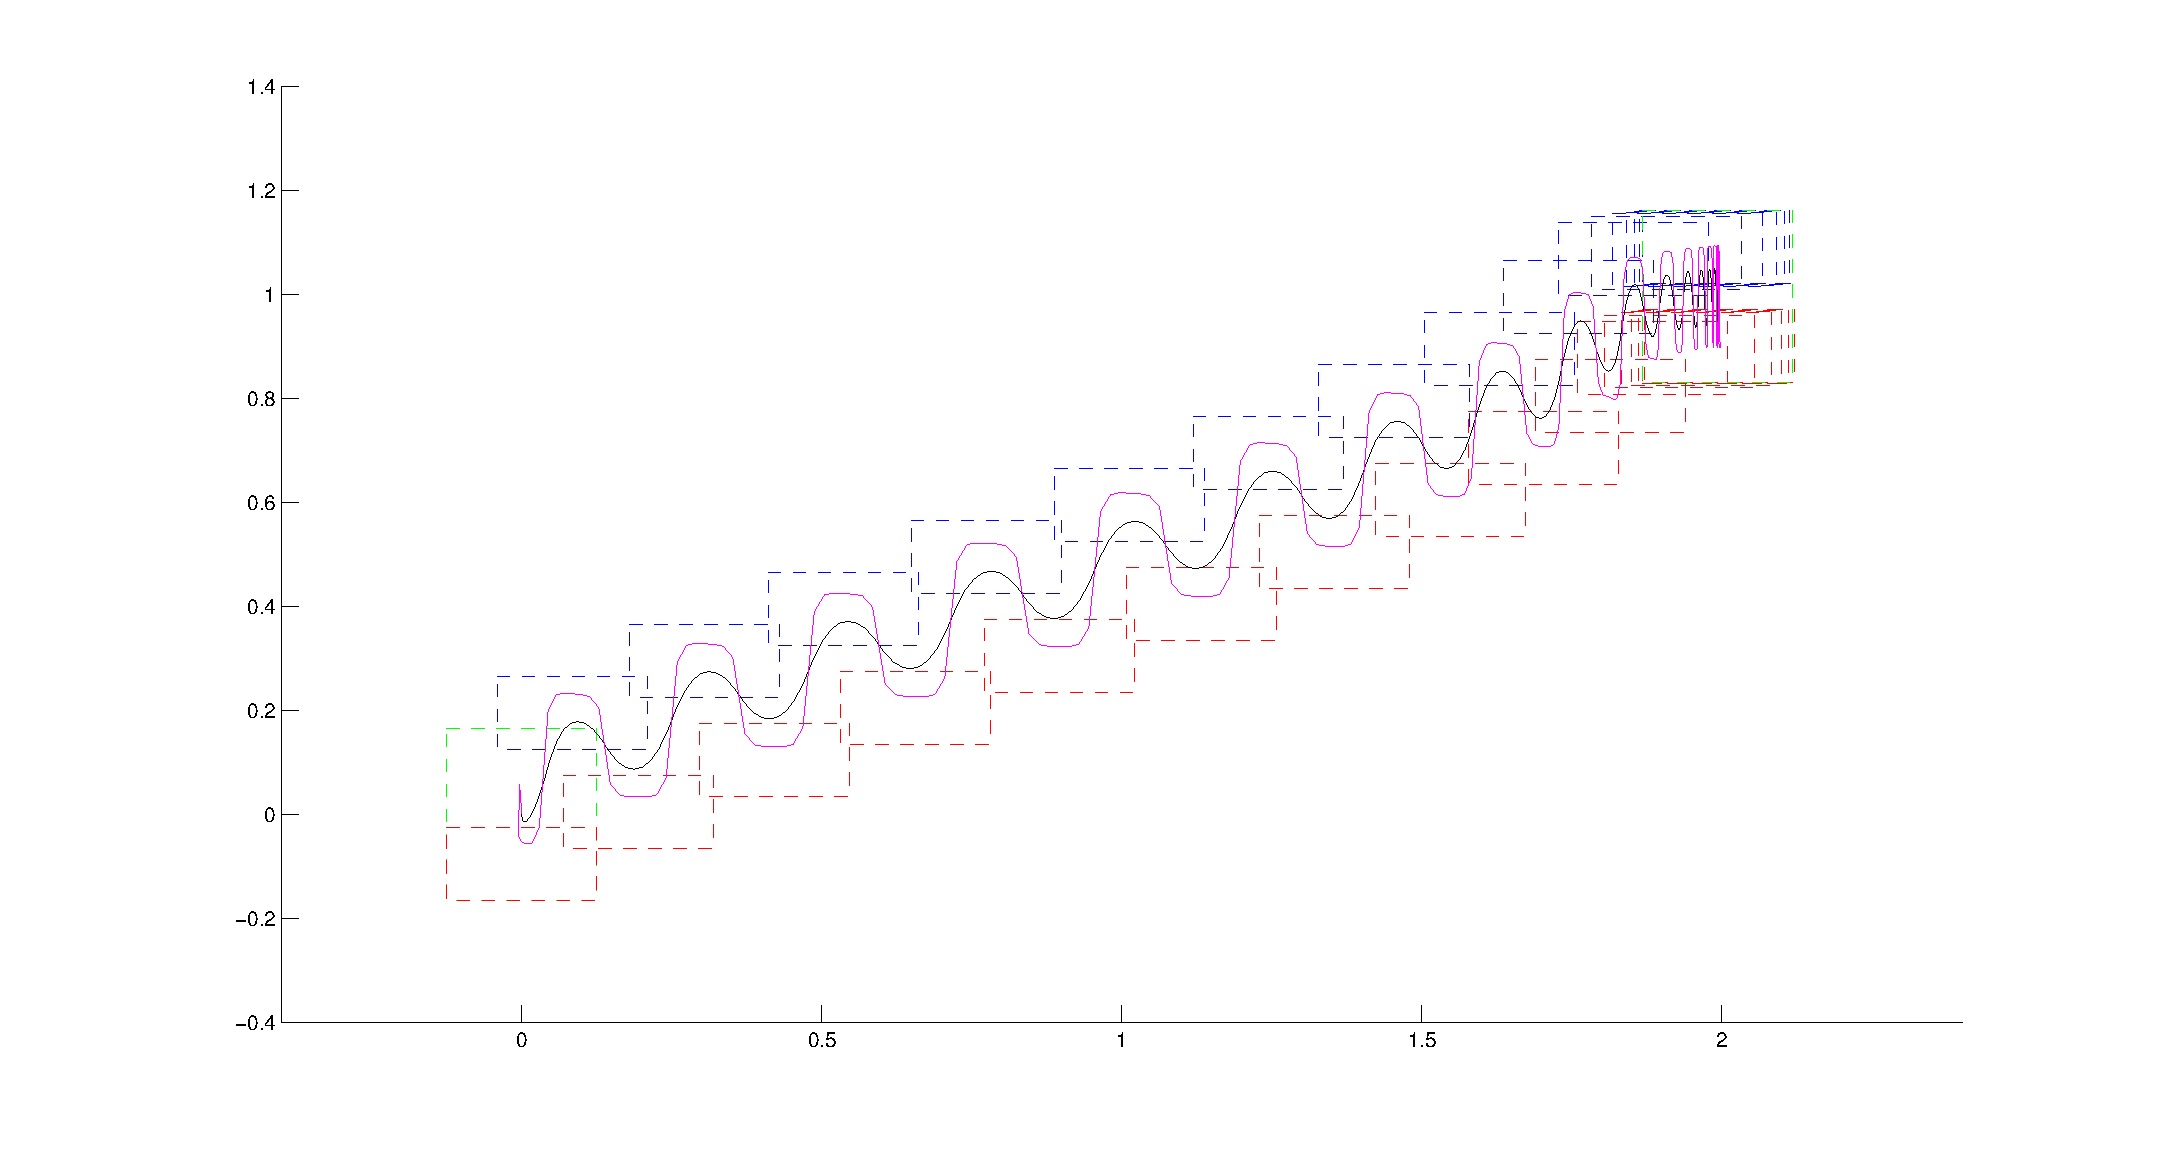
\includegraphics[scale=.25]{Chap4-Visual-Servoing/steps1_hrp2.pdf}
 %}
\end{minipage}
\begin{minipage}{0.5\textwidth}
 \centering
 %\subfigure[]{
 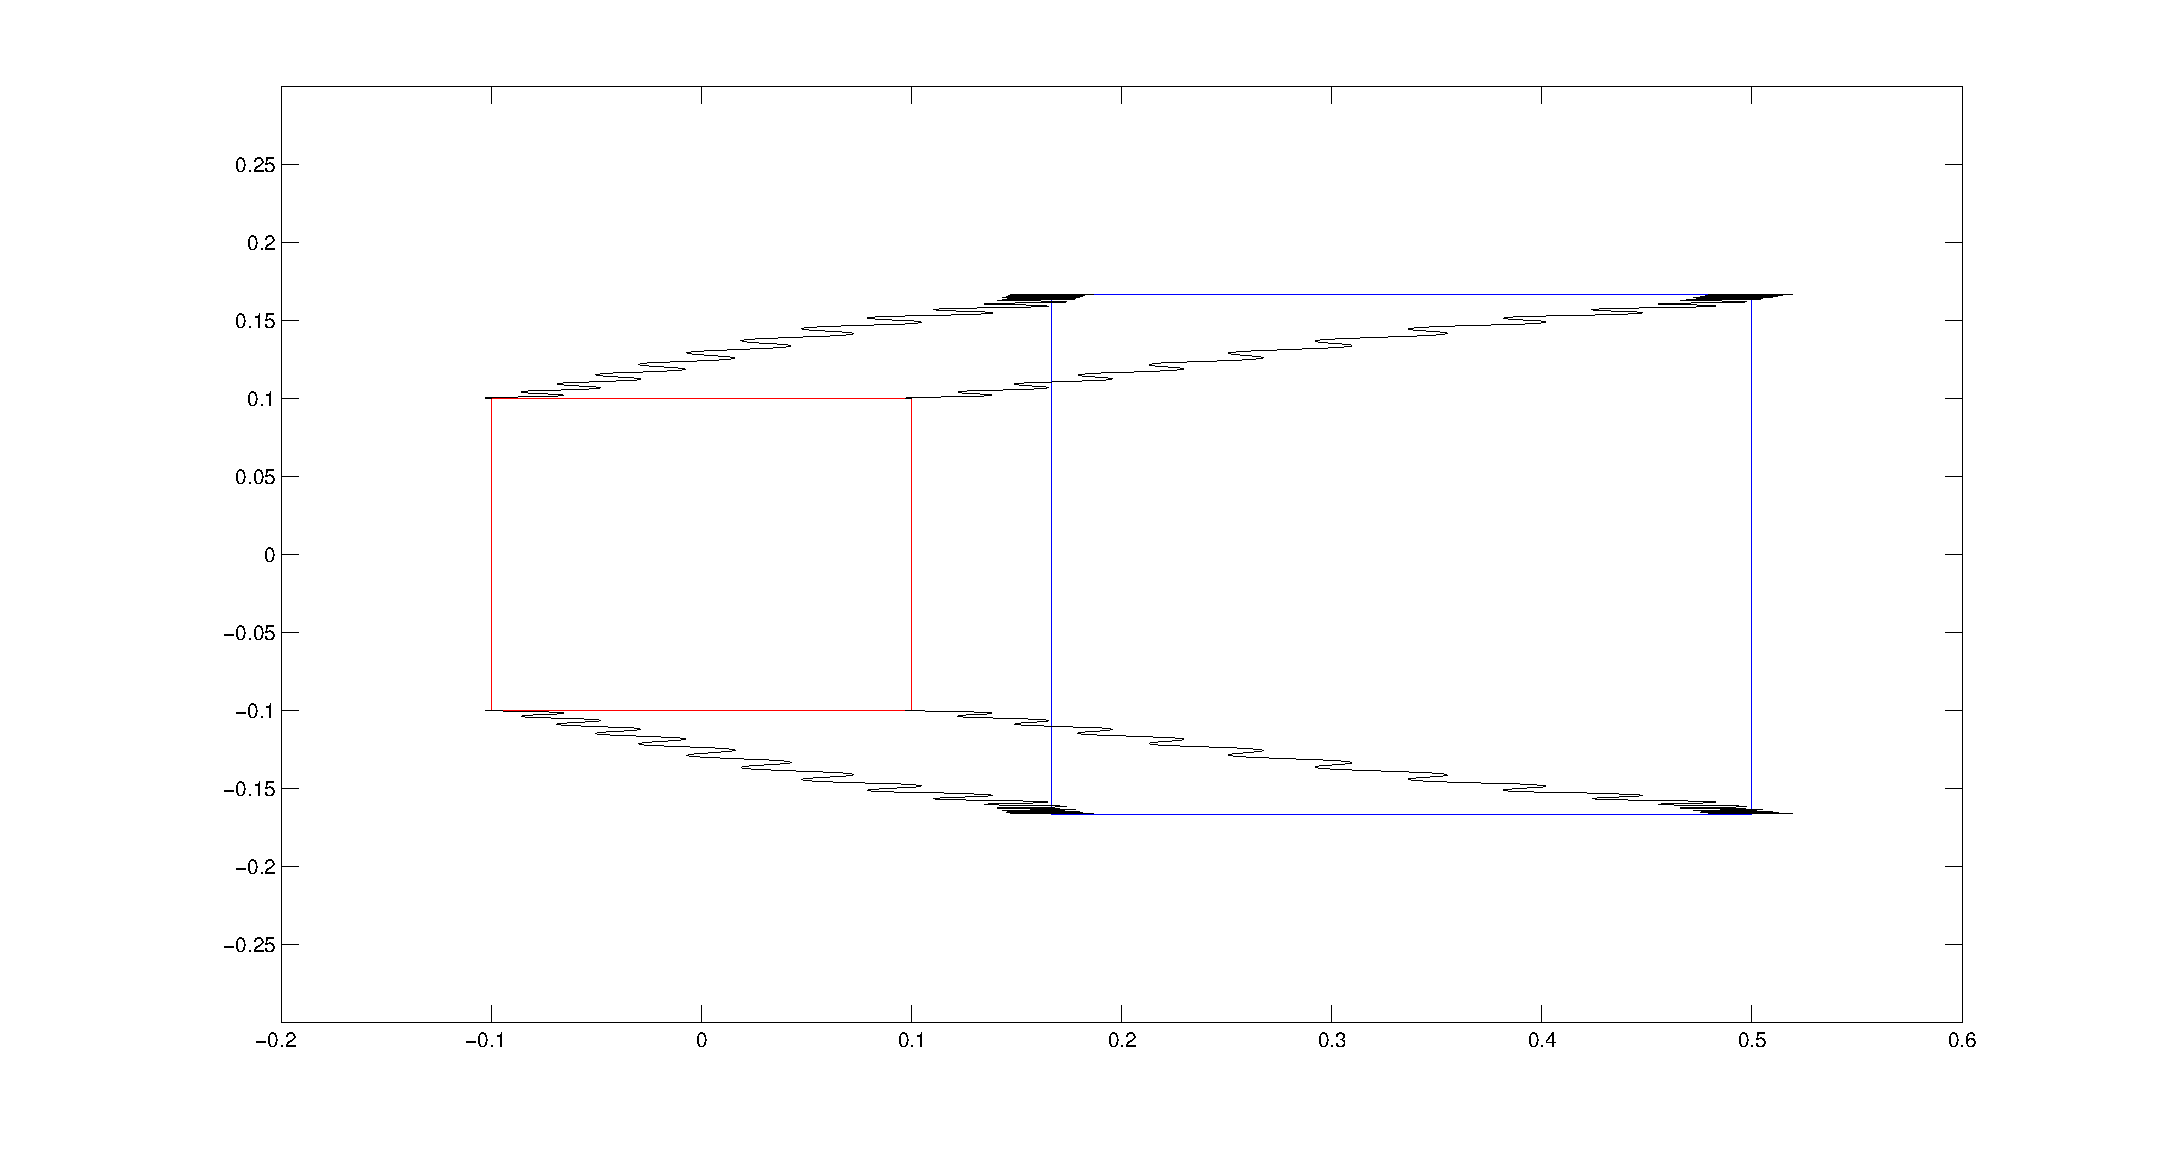
\includegraphics[width=5cm,height=4cm]{Chap4-Visual-Servoing/features1_hrp2.pdf}
 %}
\\
 %\subfigure[]{
 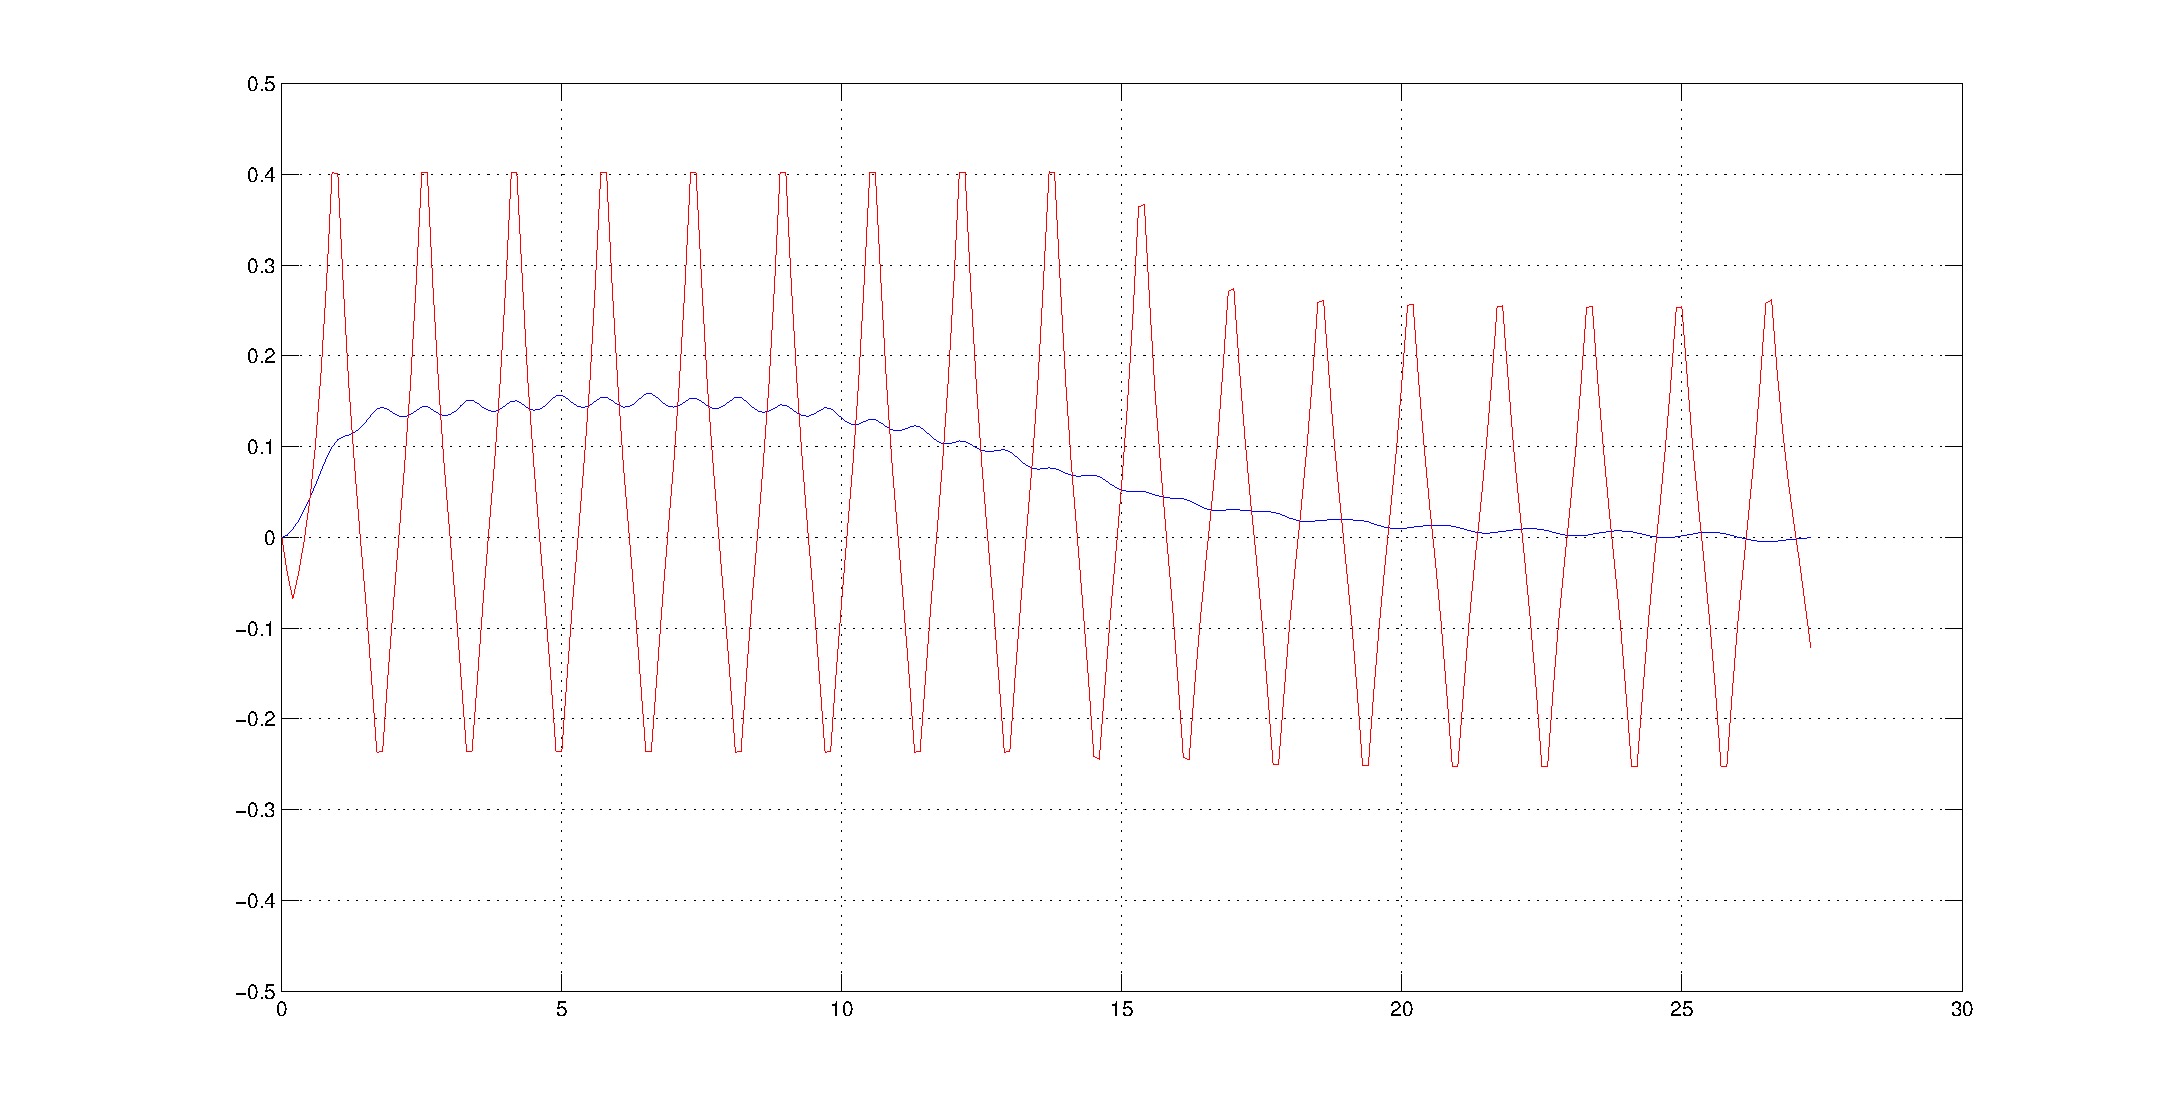
\includegraphics[scale=.2]{Chap4-Visual-Servoing/vels1_hrp2.pdf}
 %}
\end{minipage}
 \caption[]{\label{Fig:Results1}\small{On the left, we show the trajectory of the robot in the $x,y$ plane, driven by our MPC-based coupled approach. The initial and final double stance phases appear in green. The single stance support feet appear in red (resp. blue) for the right (resp. left) foot. In pink, we depicted the CoP trajectory, which can be observed to remain safely in the support polygon, and in black the CoM trajectory. On the right, top, we depict (in black) the trajectory of the features in the image, with the initial positions in red and the desired positions in blue, for the first simulation.  Finally, the evolution of the velocities is shown in the bottom. It is interesting to note the offset of the oscillatory velocity in $x$ (in blue) and $y$ (in red) due to the features errors.}}
 \end{figure*}


\begin{figure*}[h]
\begin{minipage}{0.5\textwidth}
 \centering
  %\subfigure[]{
 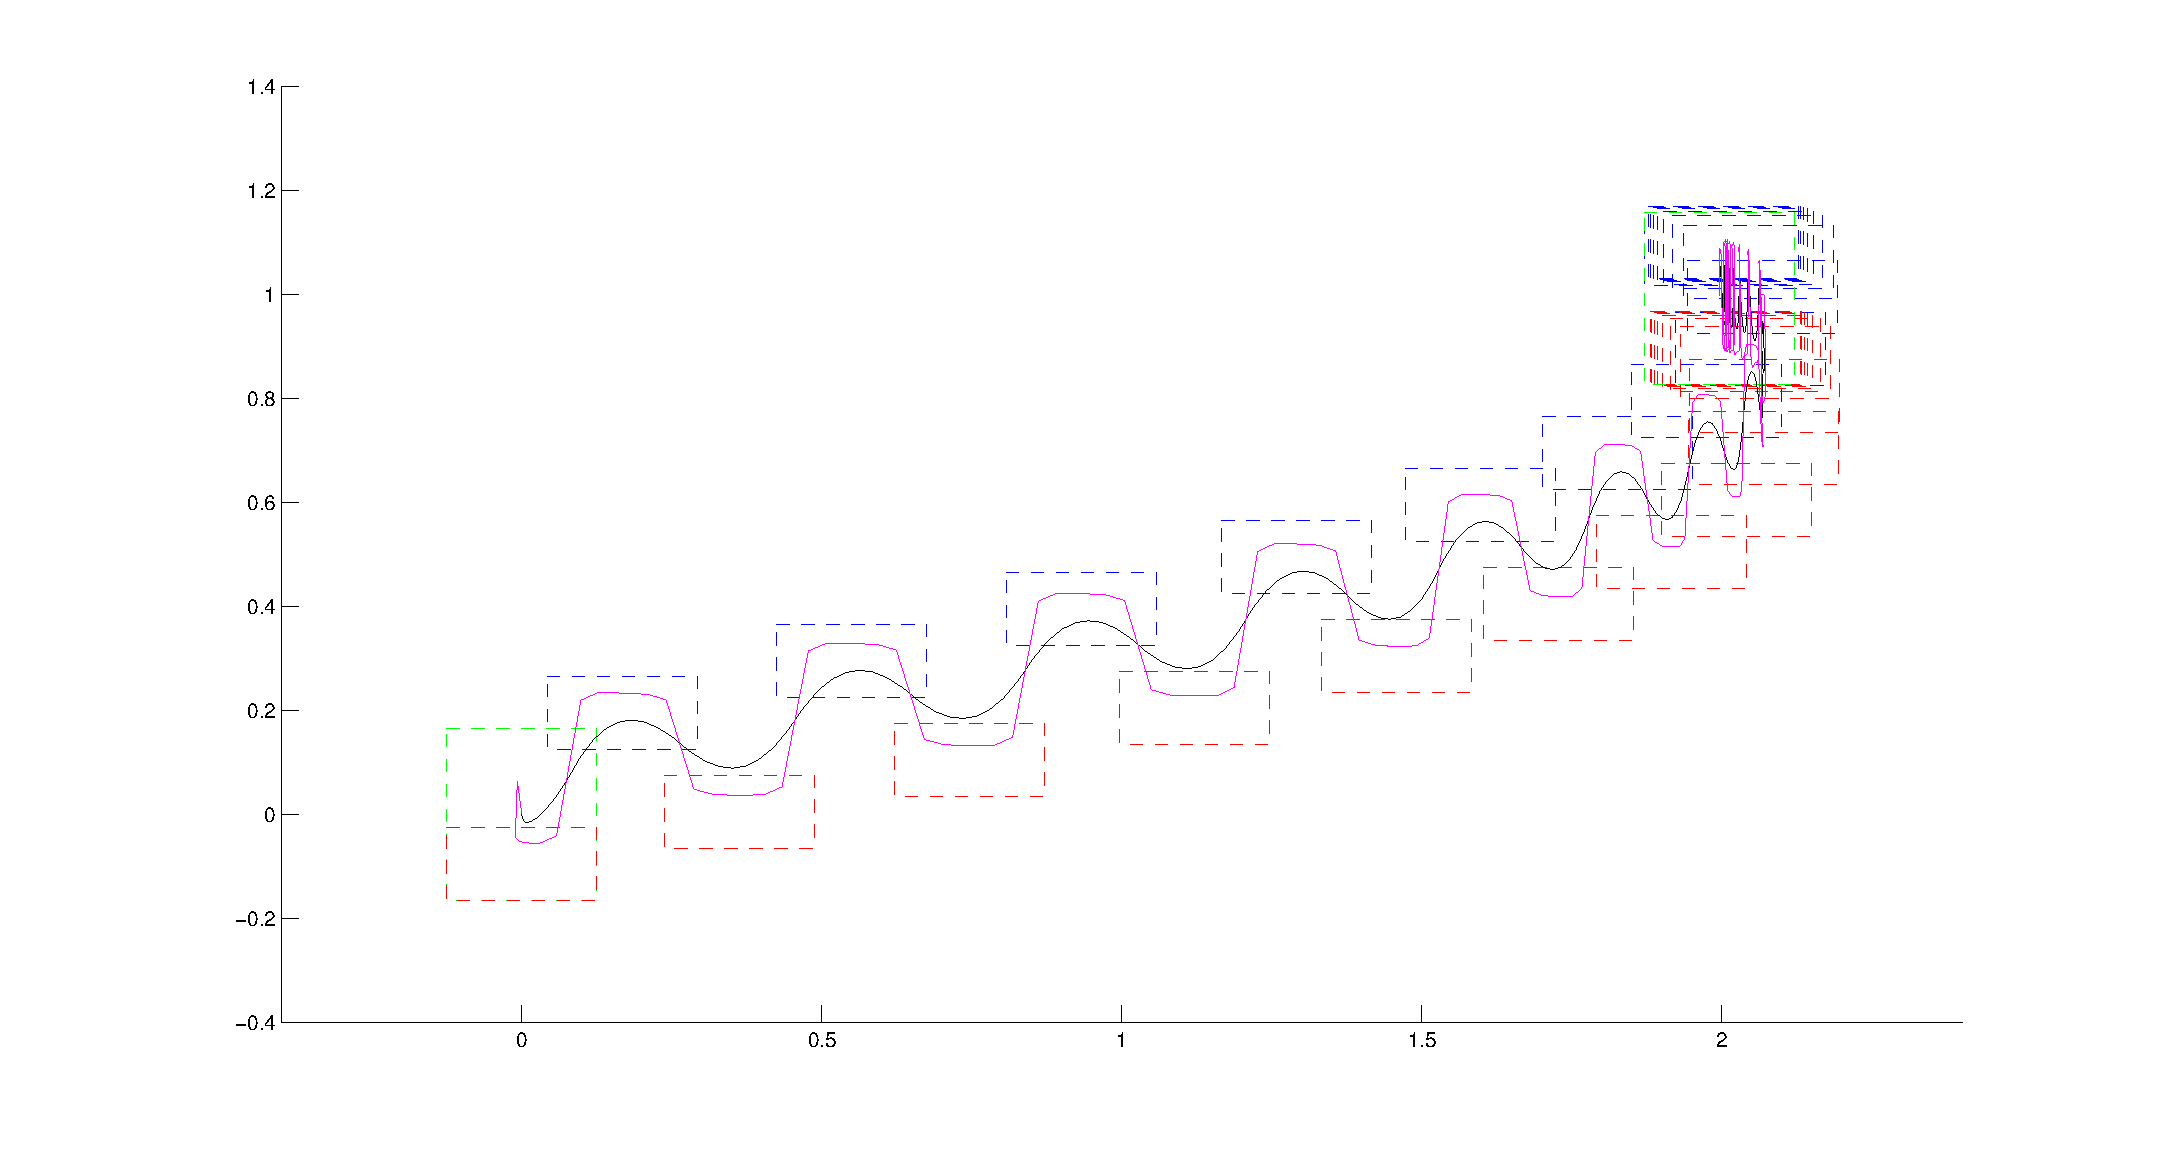
\includegraphics[scale=.25]{Chap4-Visual-Servoing/steps2_hrp2.pdf}
 %}
\end{minipage}
\begin{minipage}{0.5\textwidth}
 \centering
 %\subfigure[]{
 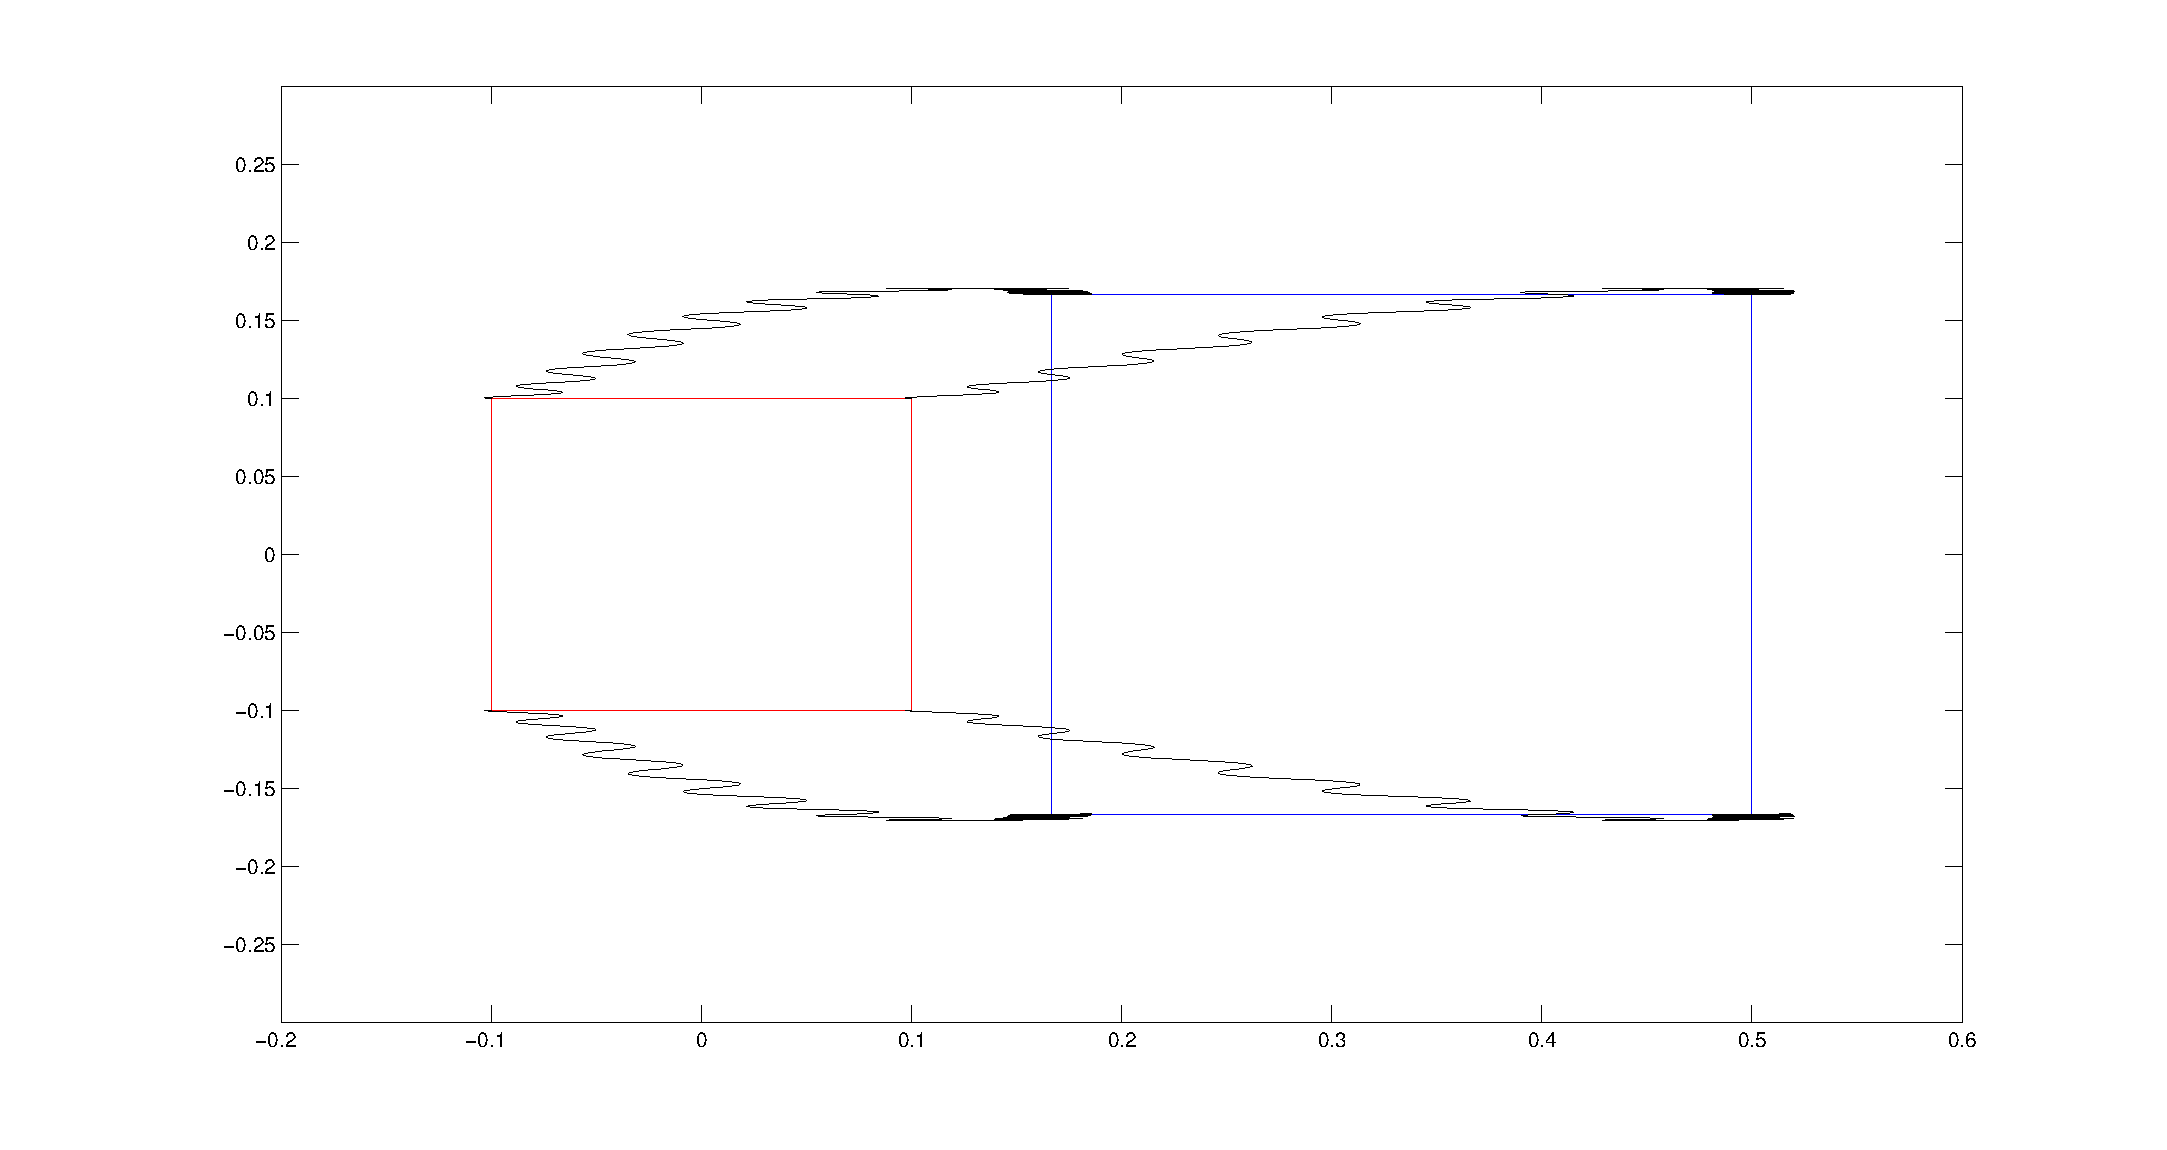
\includegraphics[width=5cm,height=4cm]{Chap4-Visual-Servoing/features2_hrp2.pdf}
 %}
\\
 %\subfigure[]{
 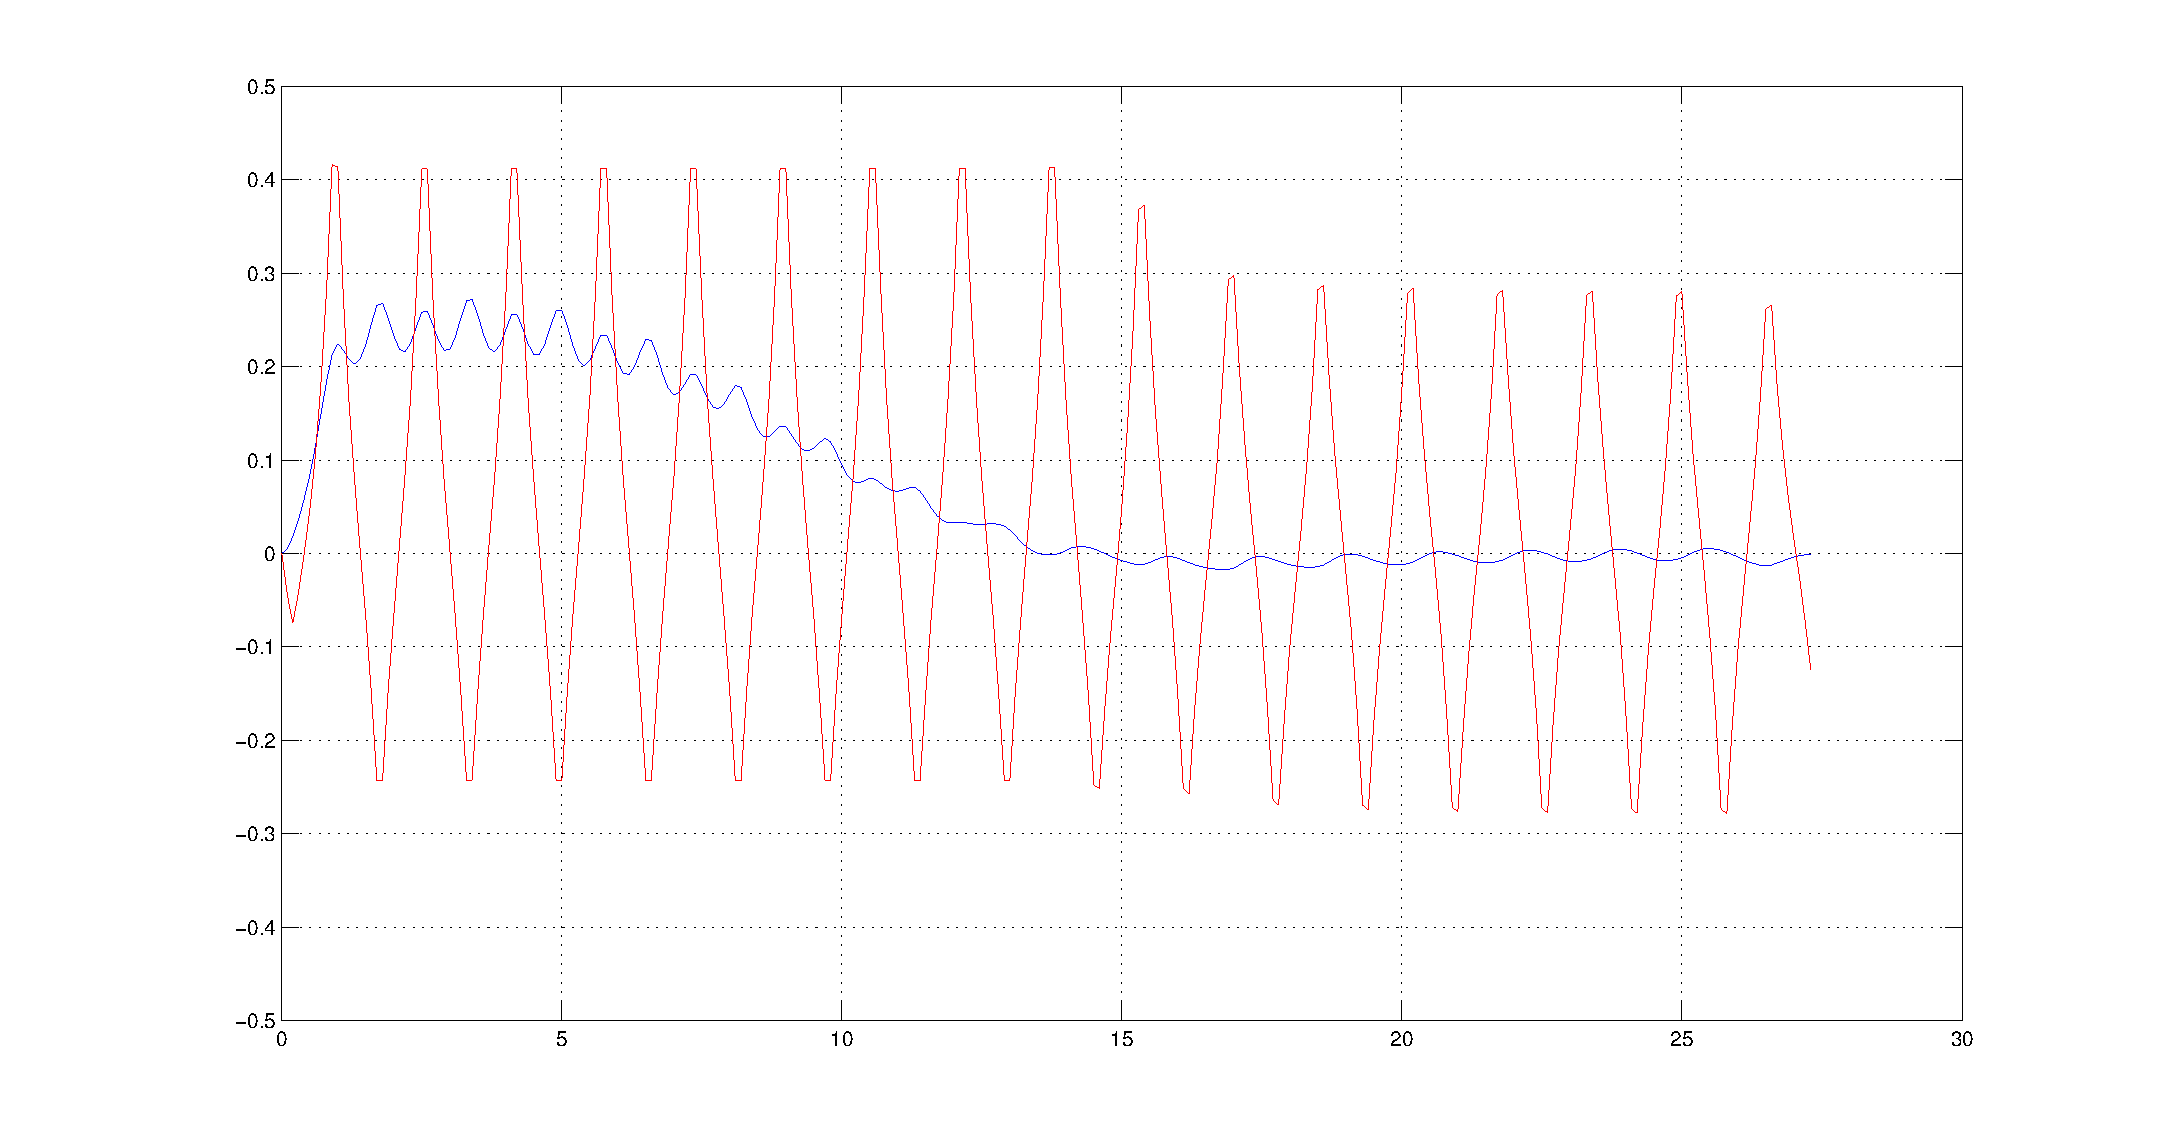
\includegraphics[scale=.2]{Chap4-Visual-Servoing/vels2_hrp2.pdf}
 %}
\end{minipage}
 \caption[]{\label{Fig:Results2}\small{The behavior of our system in the second simulation ($\beta$ is 5 times higher), with the same graphical conventions as in Fig.~\ref{Fig:Results1}. The robot is following a quite distinct trajectory, with a backwards part close to the end. As the priority is to minimize features errors, disregarding the jerks, high velocities are taken.}}
 \end{figure*}

Now, in a second experiment, we evaluate the trajectory with rotation. We recall that the rotation velocity control is decoupled from the $x$ and $y$ velocities control. It works as follows: The rotation velocity controller sets (in a decoupled way) the angular position while the main controller (QP) adapts the $x,y$ velocities in terms of these computed angular positions (which are known in the horizon), the visual errors, the footsteps centering and the jerks minimization. The results of a first simulation involving rotation is shown in Fig.~\ref{Fig:Results3}. One can observe that the dynamical balance is kept, and that most of the correction related to the rotation is done at the beginning of the trajectory. Also, in Fig.~\ref{Fig:Results4}, we can see that it is robust to perturbations: The same trajectory is followed as in Fig.~\ref{Fig:Results3} but a strong perturbation in the CoM position has been introduced (simulating an external force applying to the CoM or a string error in the position estimation), inducing visible peaks in the velocities. However, the perturbation is recovered quasi-instantly.

\begin{figure*}[h]
\begin{minipage}{0.5\textwidth}
 \centering
  %\subfigure[]{
 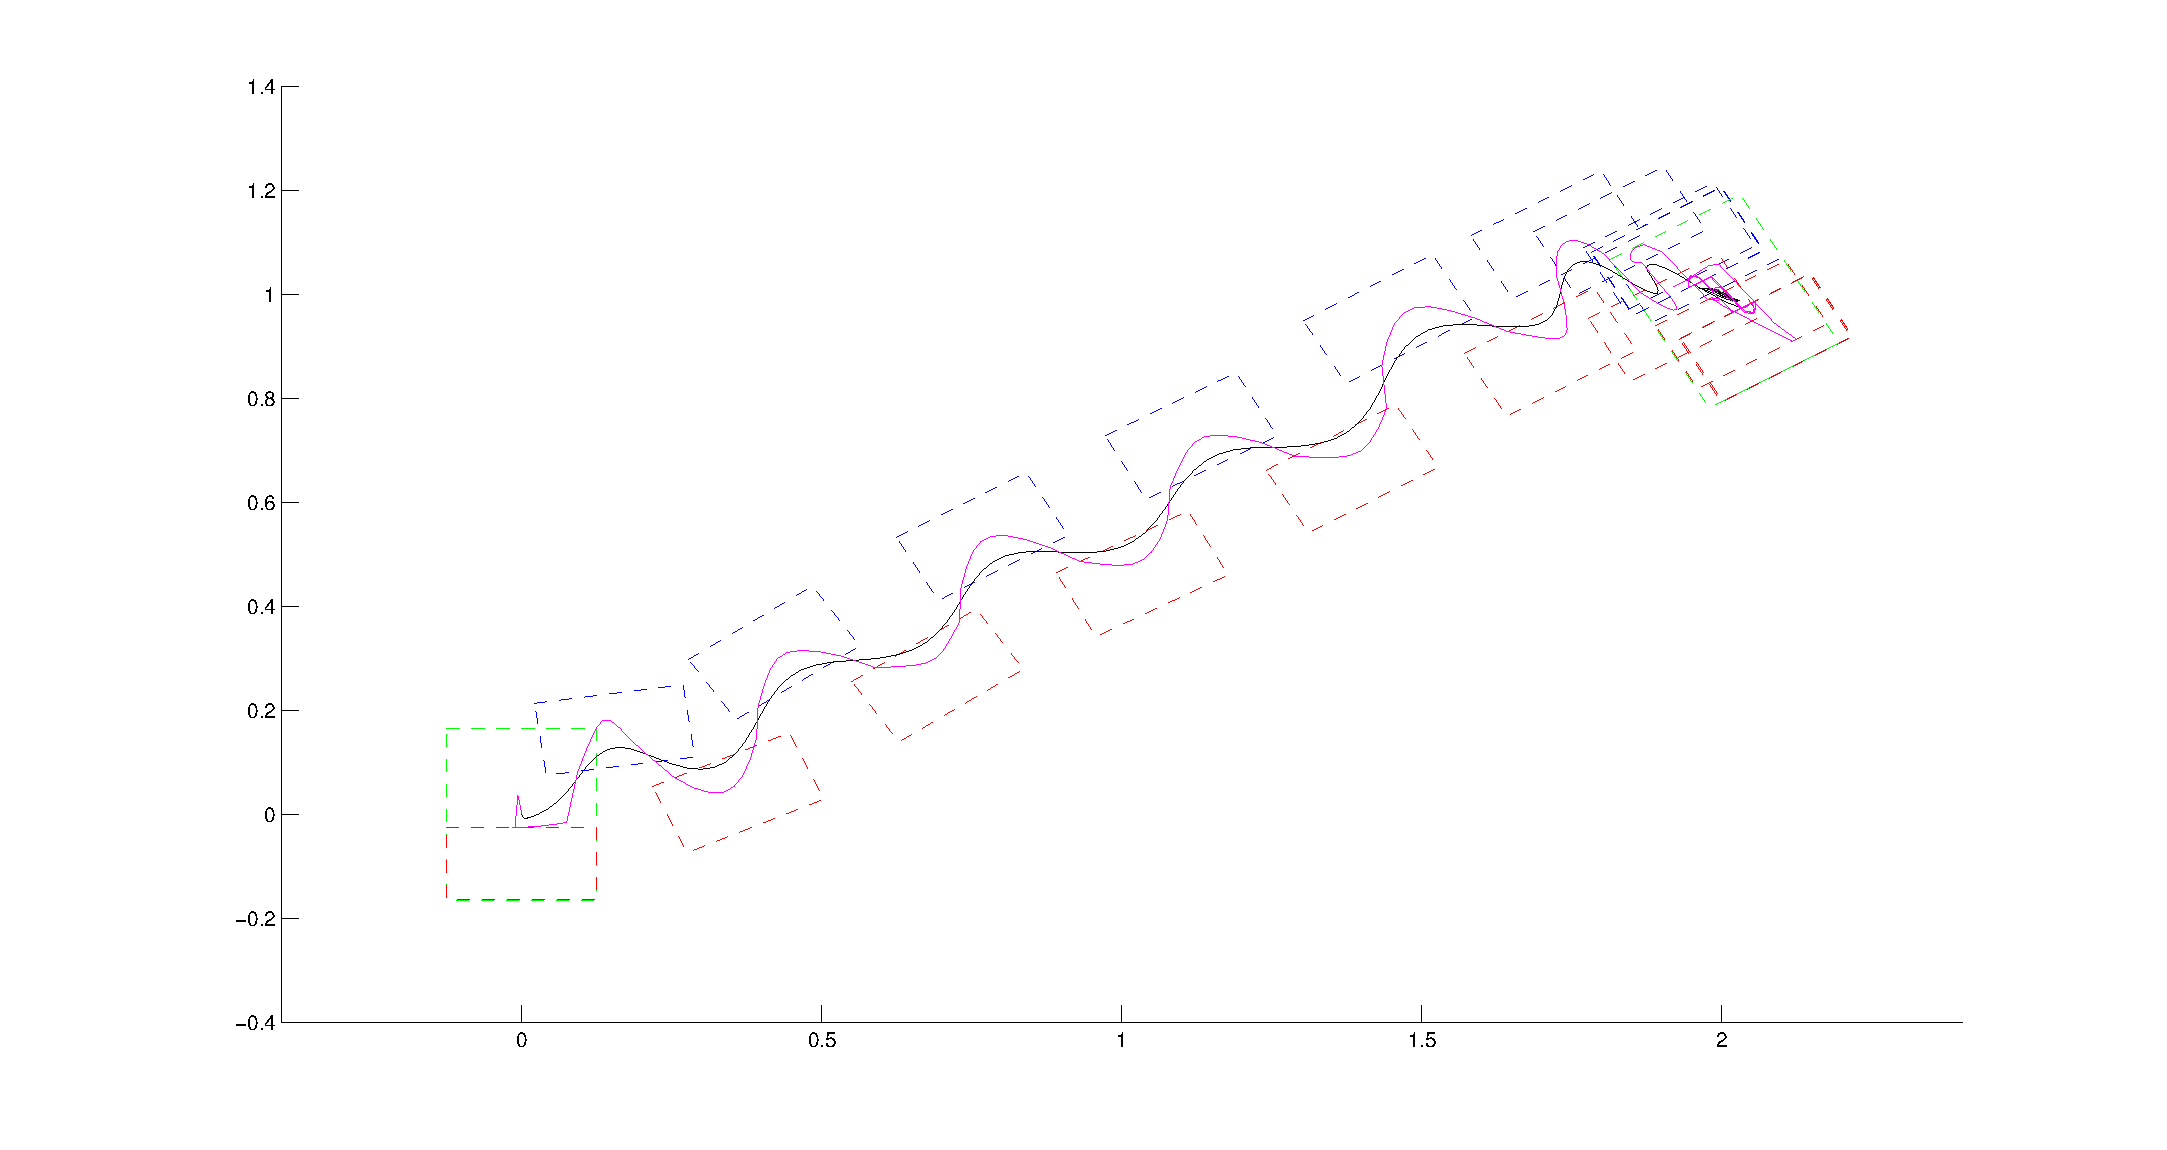
\includegraphics[scale=.25]{Chap4-Visual-Servoing/steps3_hrp2.pdf}
 %}
\end{minipage}
\begin{minipage}{0.5\textwidth}
 \centering
 %\subfigure[]{
 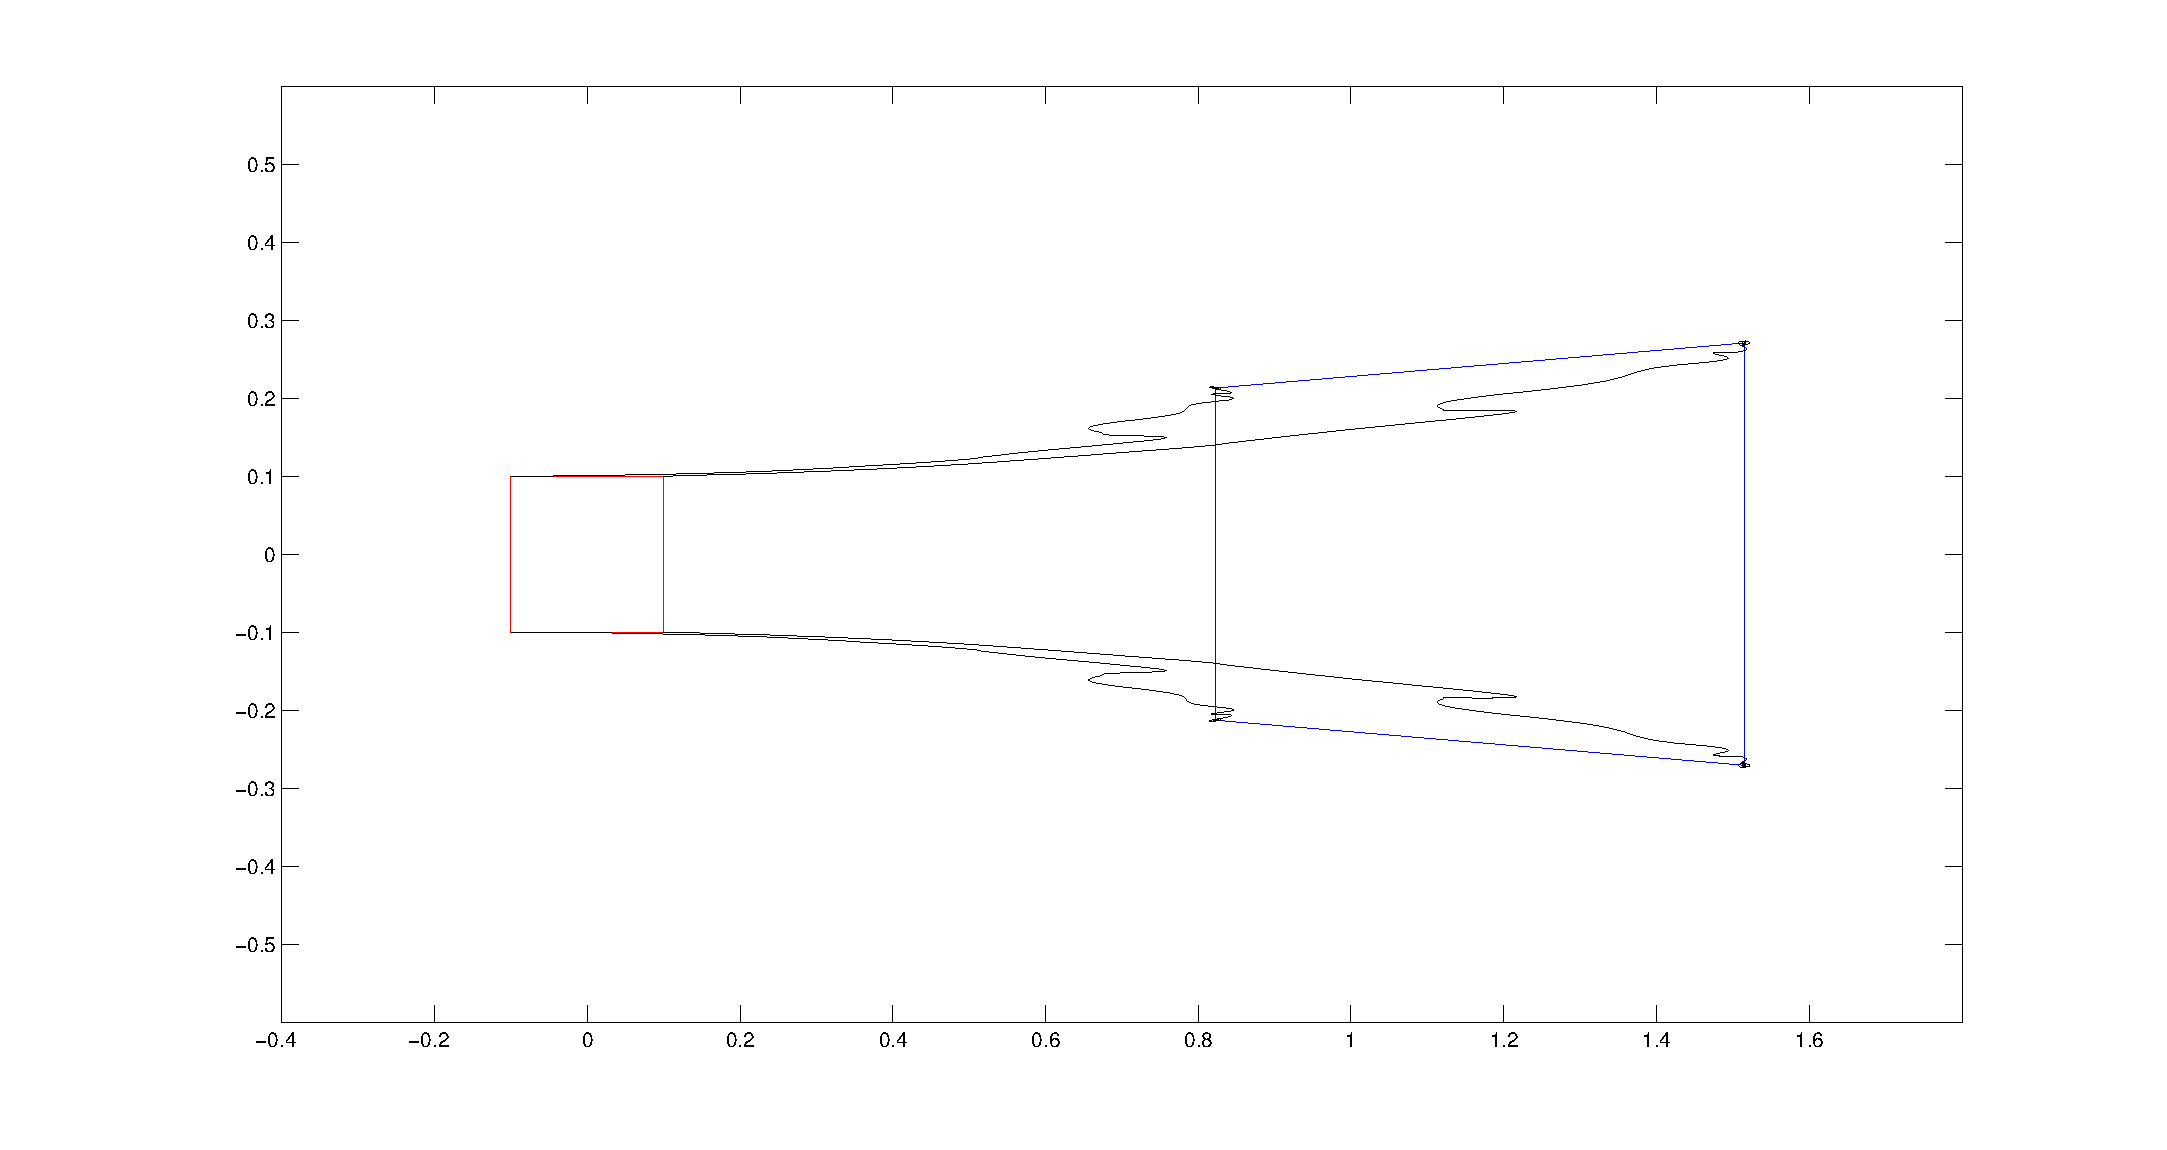
\includegraphics[width=5cm,height=4cm]{Chap4-Visual-Servoing/features3_hrp2.pdf}
 %}
\\
 %\subfigure[]{
 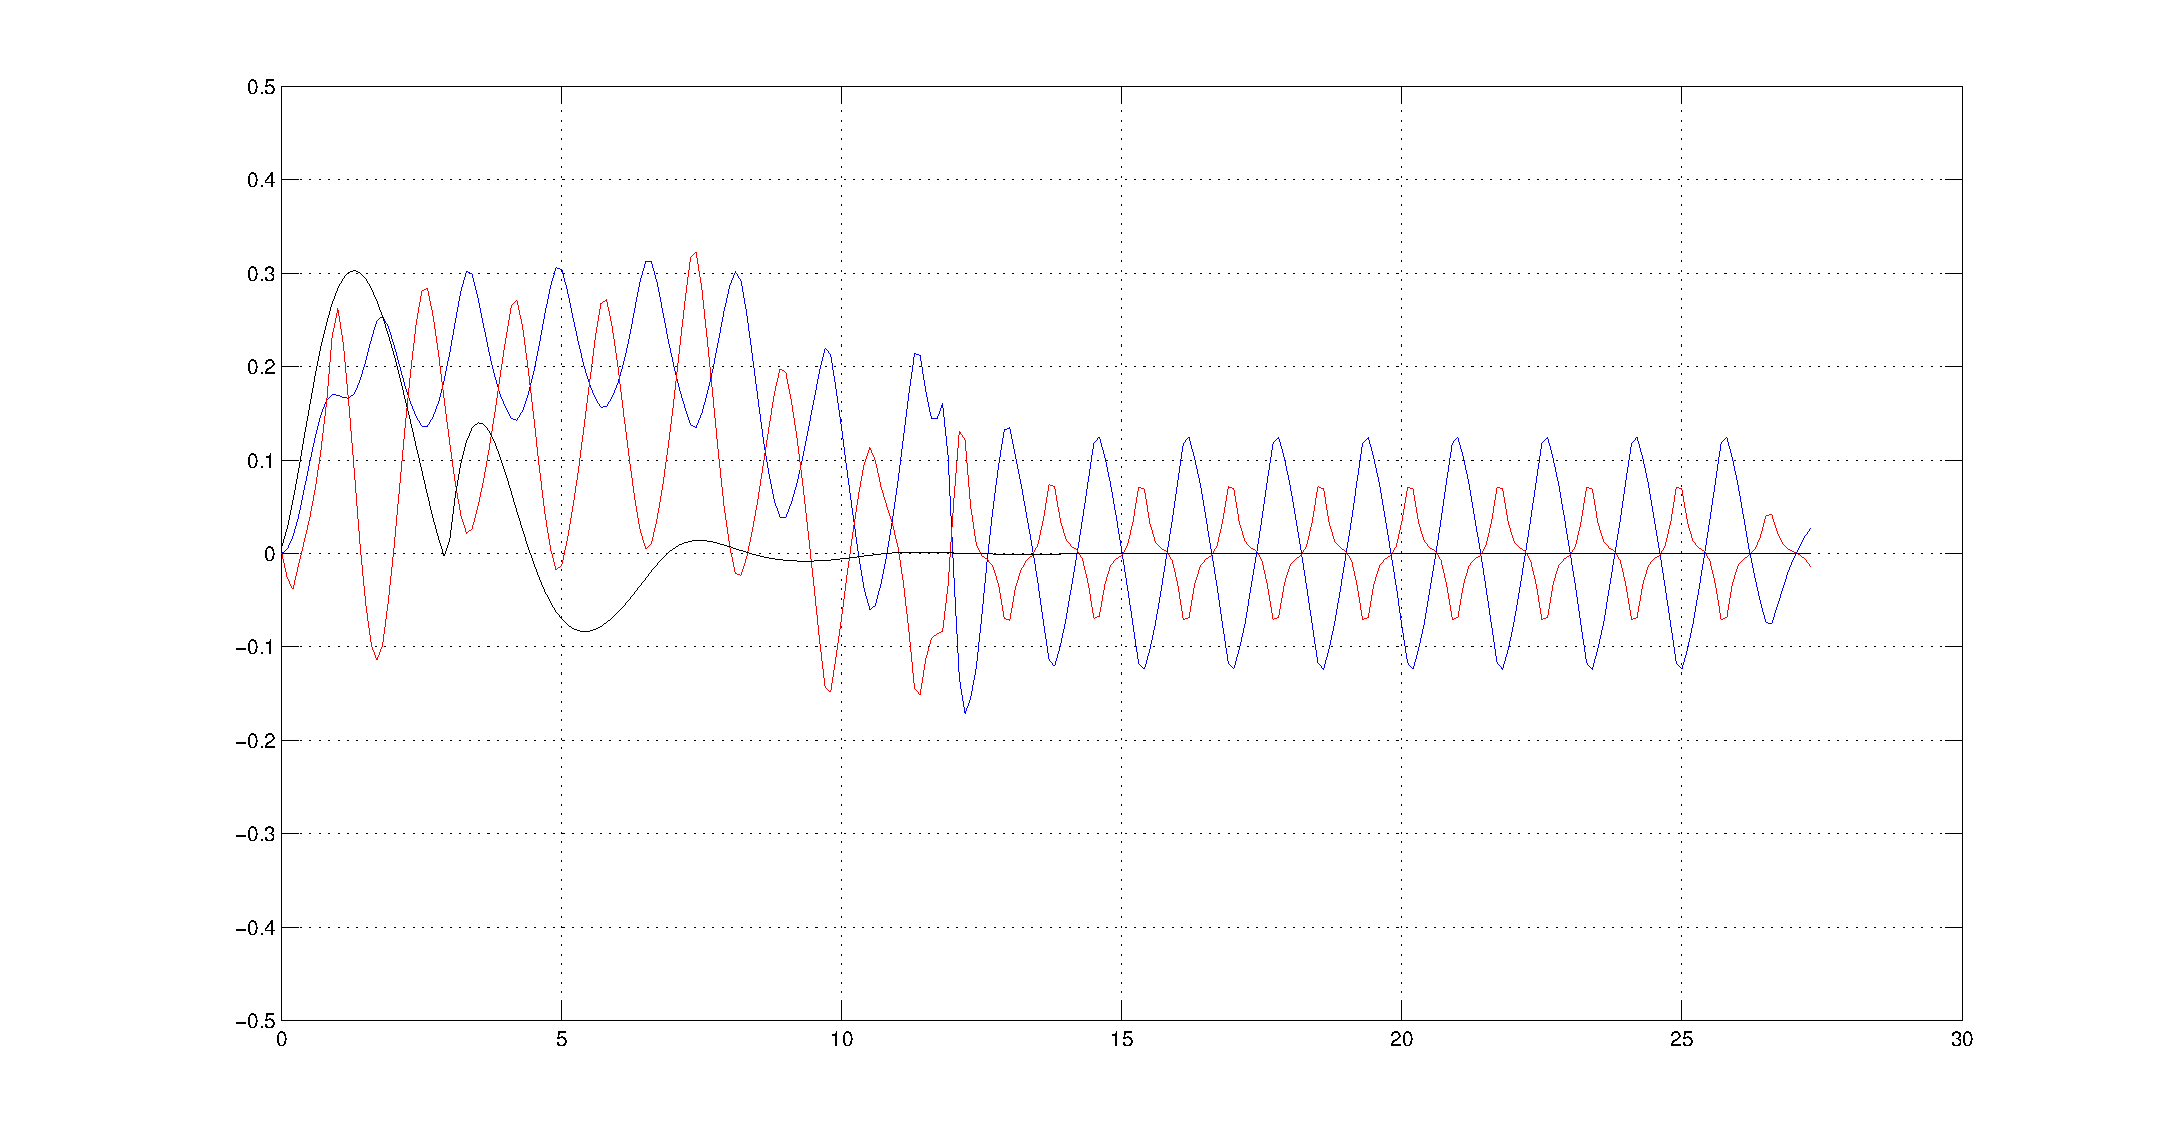
\includegraphics[scale=.2]{Chap4-Visual-Servoing/vels3_hrp2.pdf}
 %}
\end{minipage}
 \caption[]{\label{Fig:Results3}\small{The behavior of our system in the third simulation, involving rotation, with the same graphical conventions as in Fig.~\ref{Fig:Results1}. In the velocities graph (right, bottom) we added the rotation velocity in black. The robot is walking in the sagittal direction most of the time, after an initial rotation. The amplitude of the oscillations of the CoM and subsequently of the features are smaller than in the first simulation. However, we can see a non-negligible component of velocity in the positive $y$ direction, since the angle is not fully compensated. When the angle is almost fully compensated, this component disappears.}}
 \end{figure*}

\begin{figure*}[h]
\begin{minipage}{0.5\textwidth}
 \centering
  %\subfigure[]{
 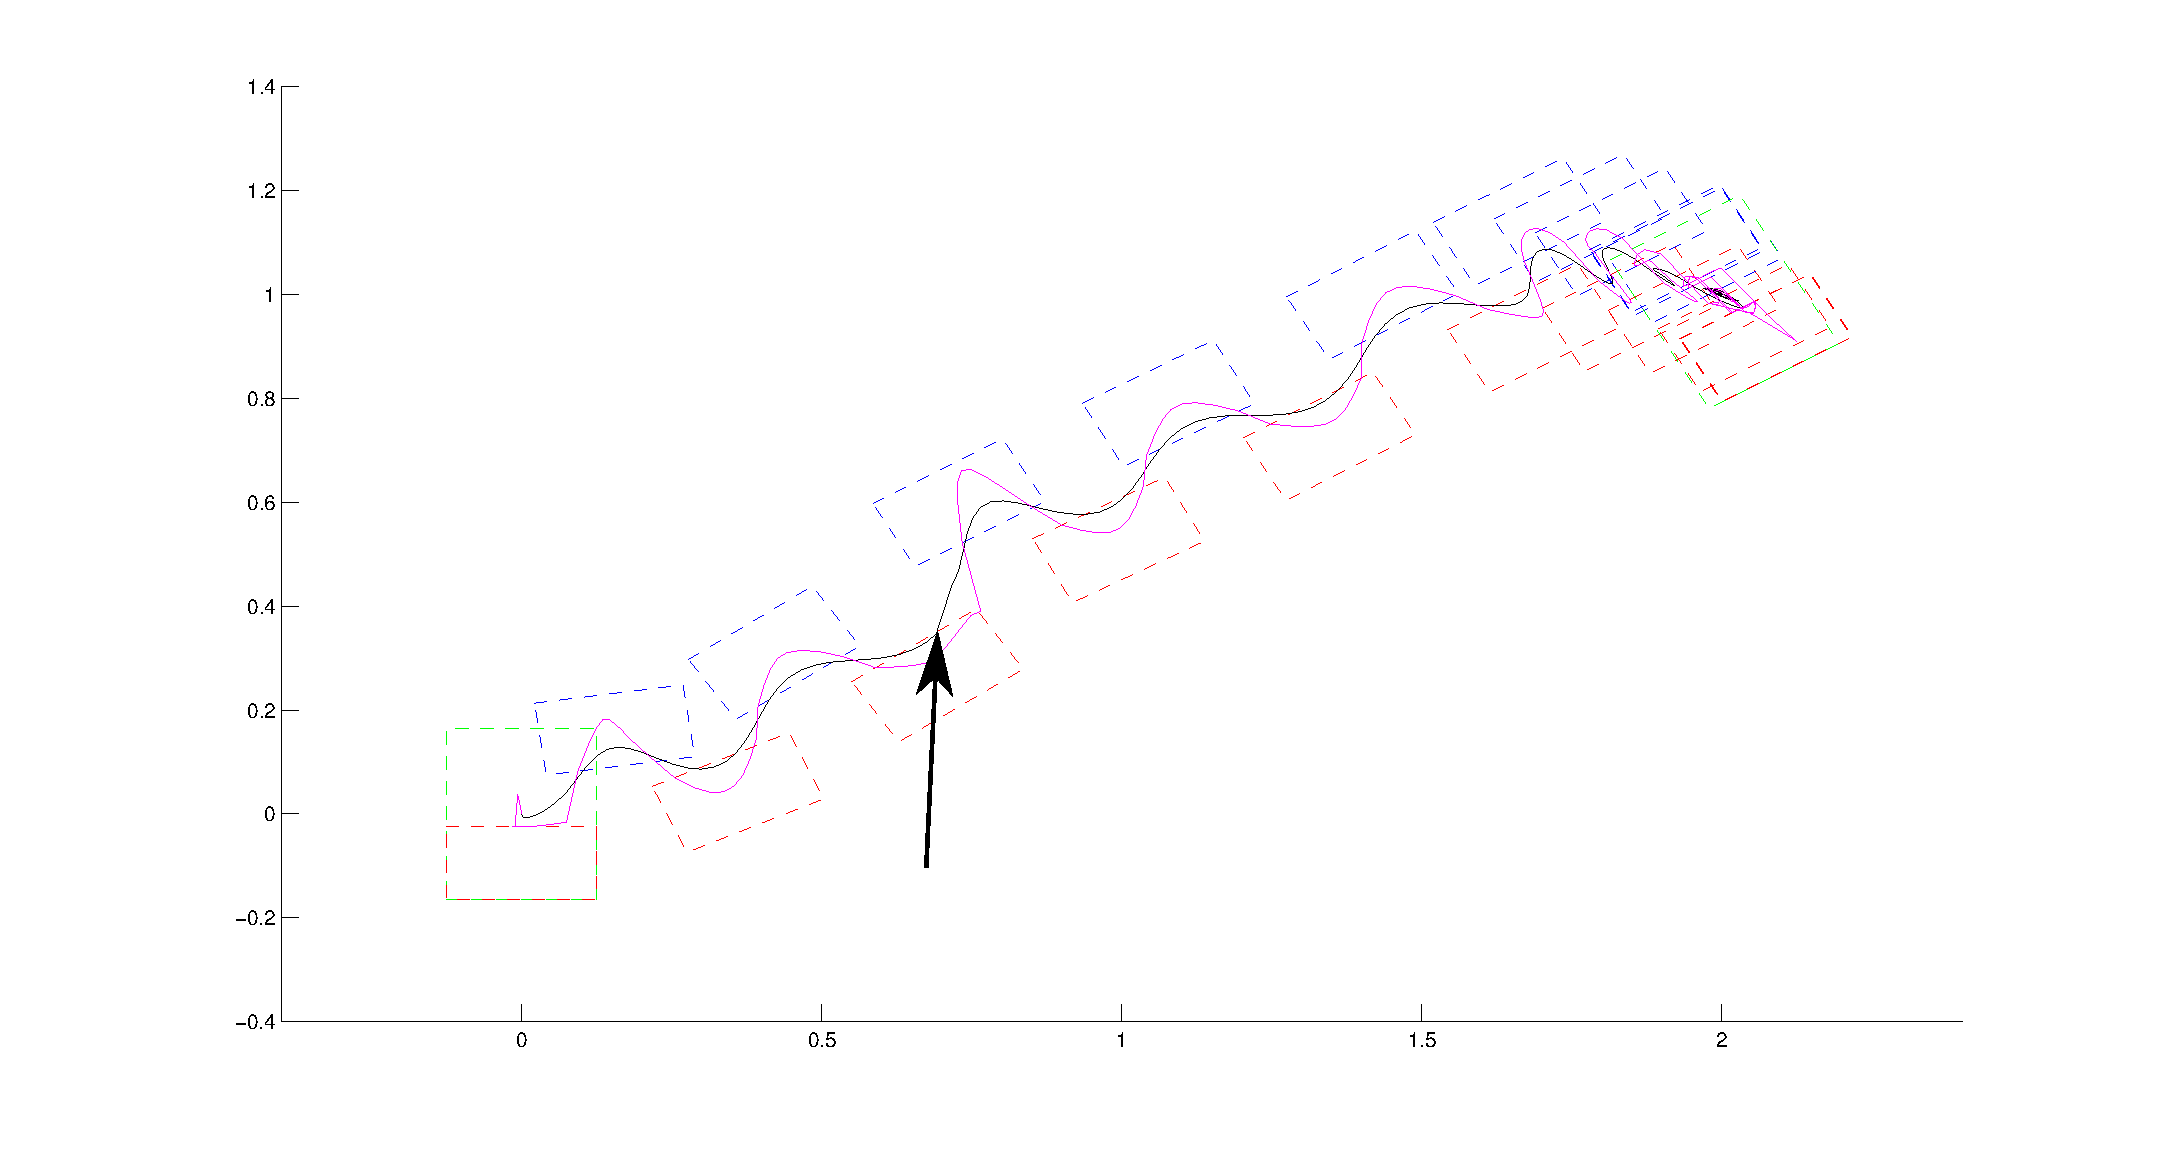
\includegraphics[scale=.25]{Chap4-Visual-Servoing/steps4_hrp2_1.pdf}
 %}
\end{minipage}
\begin{minipage}{0.5\textwidth}
 \centering
%\subfigure[]{
 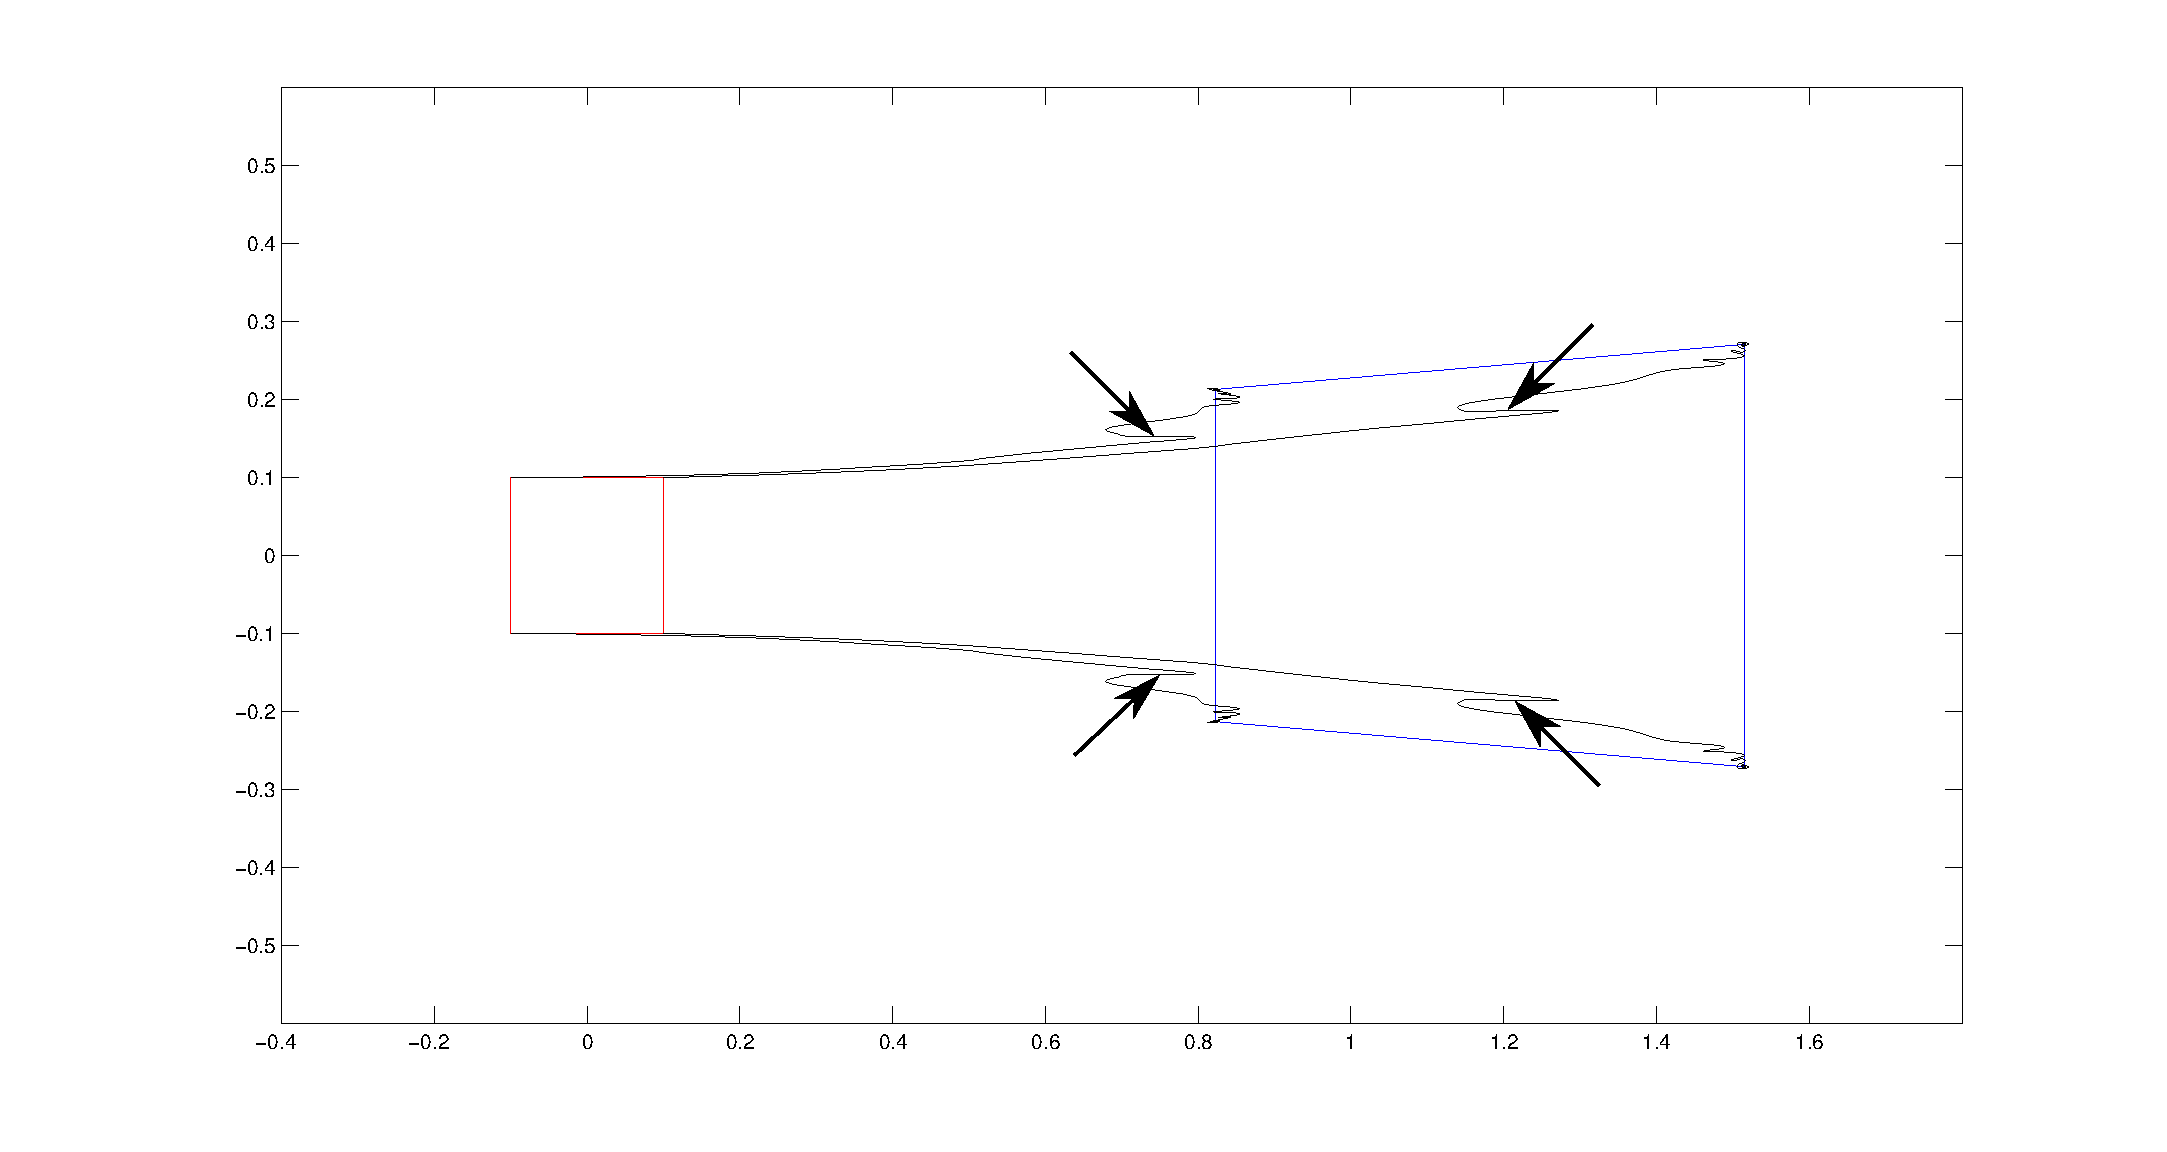
\includegraphics[width=5cm,height=4cm]{Chap4-Visual-Servoing/features4_hrp2_1.pdf}
 %}
\\
 %\subfigure[]{
 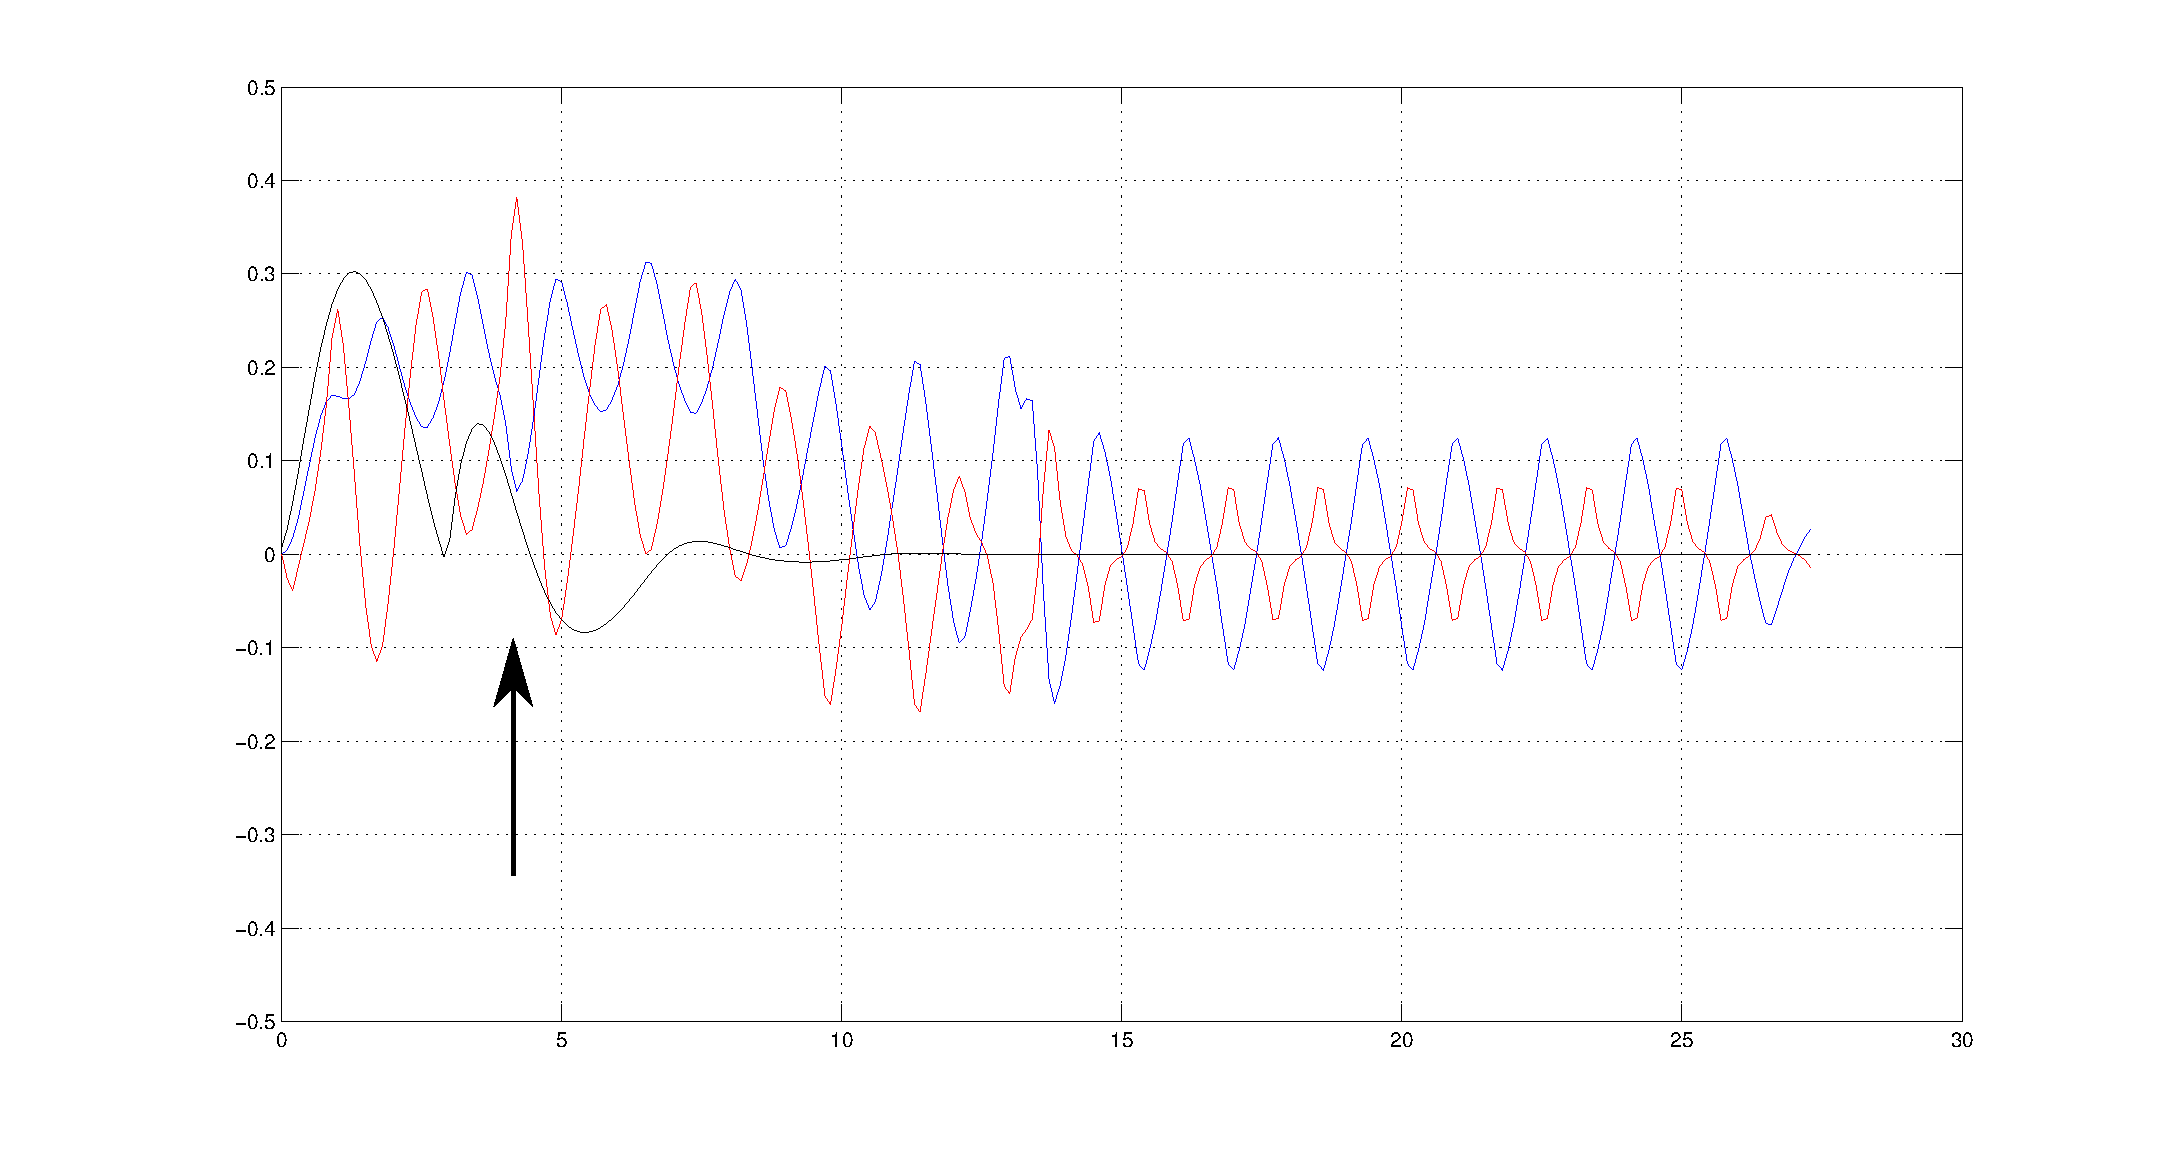
\includegraphics[scale=.2]{Chap4-Visual-Servoing/vels4_hrp2_1.pdf}
 %}
\end{minipage}
 \caption[]{\label{Fig:Results4}\small{The behavior of our system in the fourth simulation, with the same graphical conventions as in Fig.~\ref{Fig:Results3}. The robot is following a trajectory similar to the one of Fig.~\ref{Fig:Results3}. After a few footsteps, a strong perturbation is applied to the CoM, inducing a peak in the velocities graph (right, bottom). This perturbation is small in distance metric, so it is not visible in the features trajectories. The perturbation is quasi-instantly recovered.}}
 \end{figure*}

We have already explained how a local linearization is made to maintain the QP formulation. The performance of this linearization depends of the distance traveled inside the horizon, which depends on the velocity of the robot and the size of the horizon. In Fig.~\ref{Fig:Results5}, we can see the linearized and real features trajectories for a given CoM trajectory. As expected, close to the beginning (the linearization point) the trajectories are quite similar, while the final positions differ more. This is an extreme situation, since usual metric displacements in the horizon are much smaller than this one. In any case, horizon displacements are bigger when the visual errors are bigger (the robot is far from the desired position) in which case the robot just needs a tendency. But when the errors are getting smaller, the robot needs more precision. In this case, the displacements in the horizon becomes smaller so that the difference between the real model and the linearized one becomes negligible.

\begin{figure}[h]
 \centering
 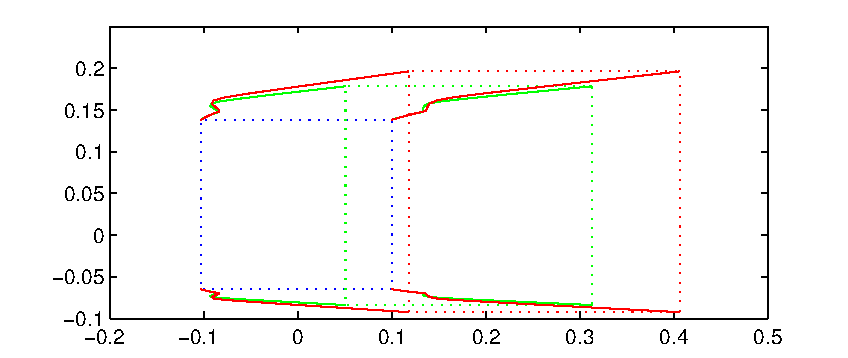
\includegraphics[scale=.8]{Chap4-Visual-Servoing/comparison_linearization}
 \caption{\label{Fig:Results5}\small{In this figure, we show the trajectory of the visual features in one iteration of the QP, and compare the evolution of the features obtained by the linearization model (green lines) and features obtained by the exact non-linear model (red lines).}}
 \end{figure}

Due to the walking nature, we have oscillations in the features trajectories. One of the main advantages of using MPC is that it naturally filters out these oscillations because we minimize the errors in a full cycle. It is remarkable that, in comparison with the decoupled approach ~\citep{DuneIROS2010} we do not need to model explicitly the sway motion of the robot and the resulting motion of the visual features. The system could oscillate inside the horizon (and it does), but at the end, the optimal control is taken without oscillations (Fig.~\ref{Fig:Results6}). In Fig.~\ref{Fig:Results6}, we only show three features errors evolution, the $u$ component of each left (black) and right (red) lower side corners, since the upper ones are, by symmetry, the same. And we complete with a single $v$ component (blue) for all the corners, with the same symmetry argument. 

\begin{figure}[ht]
 \centering
 %\subfigure[]{
 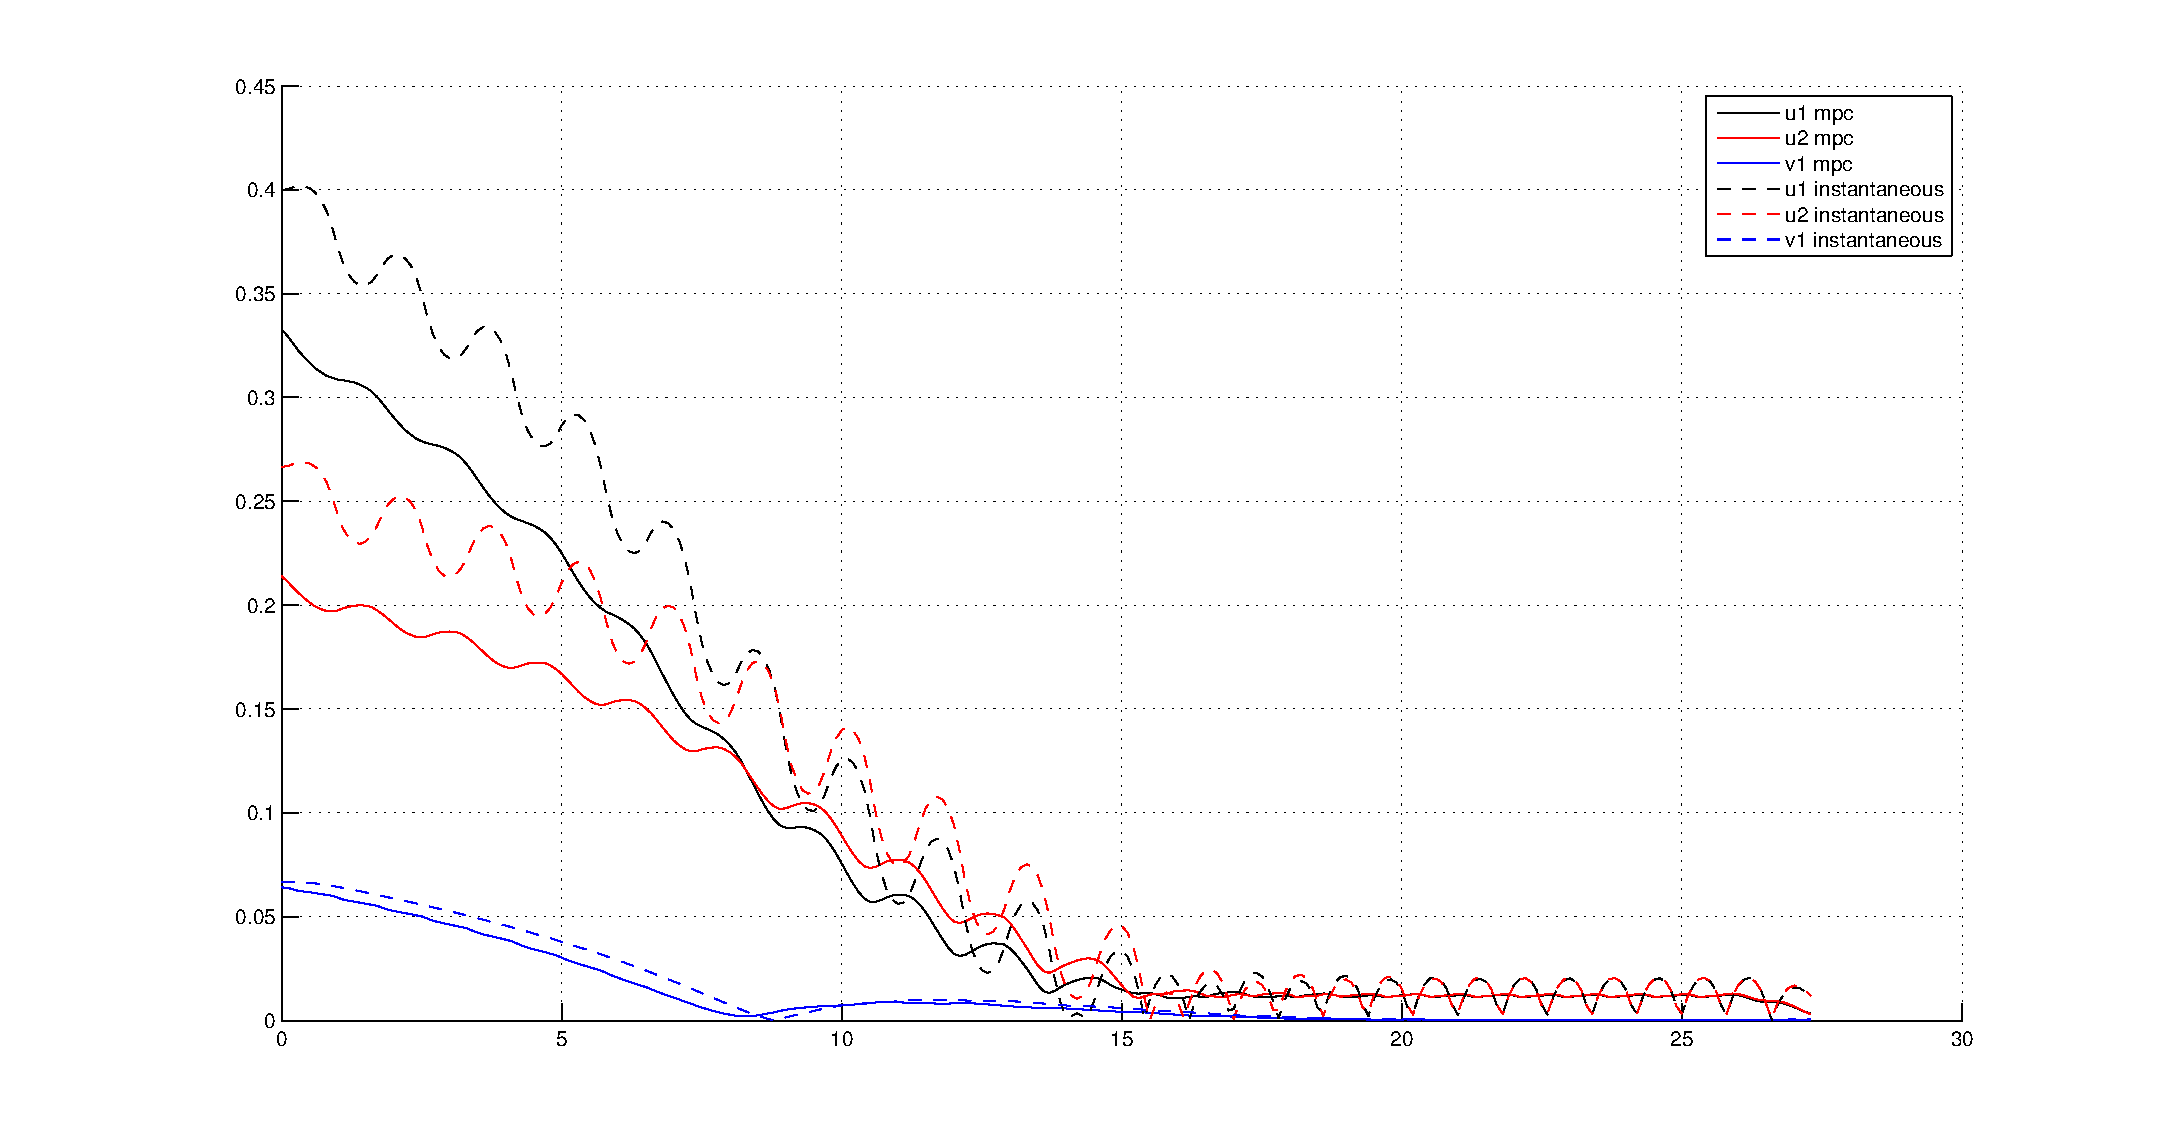
\includegraphics[scale=.35]{Chap4-Visual-Servoing/errors_mpc_instantaneous}
 \label{Fig:Results6a}
 %}
 % \subfigure[]{
 %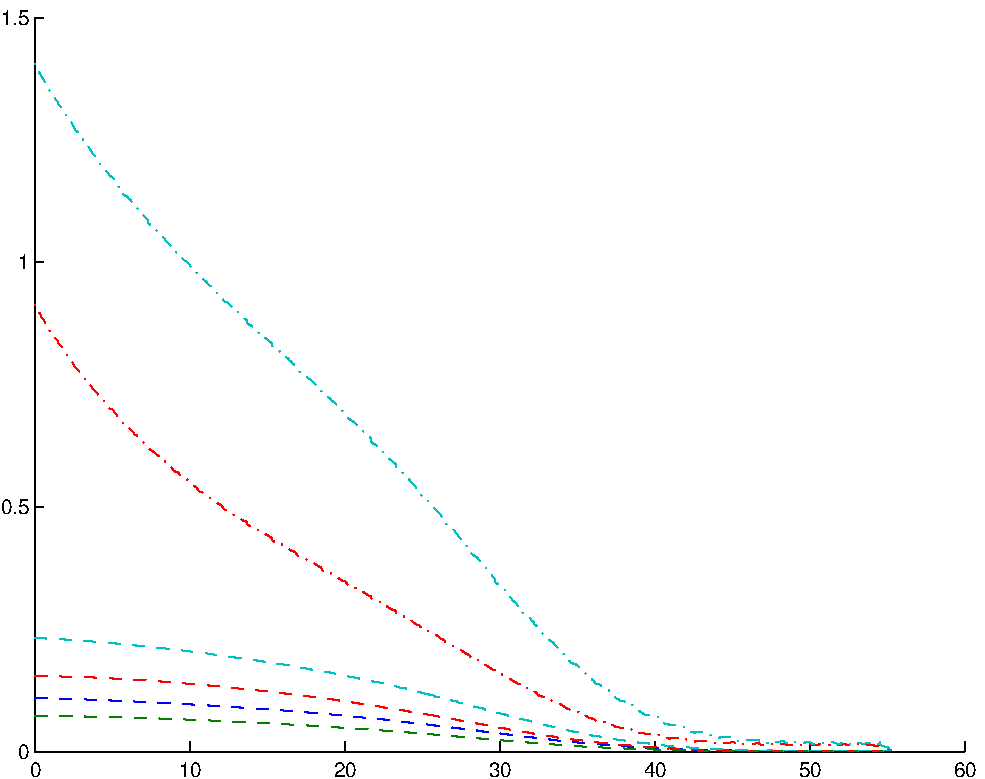
\includegraphics[scale=.23]{./figures/horizon_errors}
 %\label{Fig:Results6b}
 %}
 \caption[]{\label{Fig:Results6}\small{Evolution of the errors for the $u,v$ components of each feature, in the second simulation. In dashed line, we depict the instantaneous errors along time, and in solid line, we depict the errors estimated in the horizon (i.e. individual terms of Eq.~ \ref{Eq:MinVisualFeatures2}, normalized by the size of the horizon). Observe that the sway motion of the robot induces oscillations of the $u$ components in the instantaneous errors, and that these oscillations are not present in the errors estimated in the horizon window.}}
 \end{figure}

\subsection{Comparisons: coupled vs. decoupled approaches}

\begin{figure*}[ht]
 \centering
 \subfigure{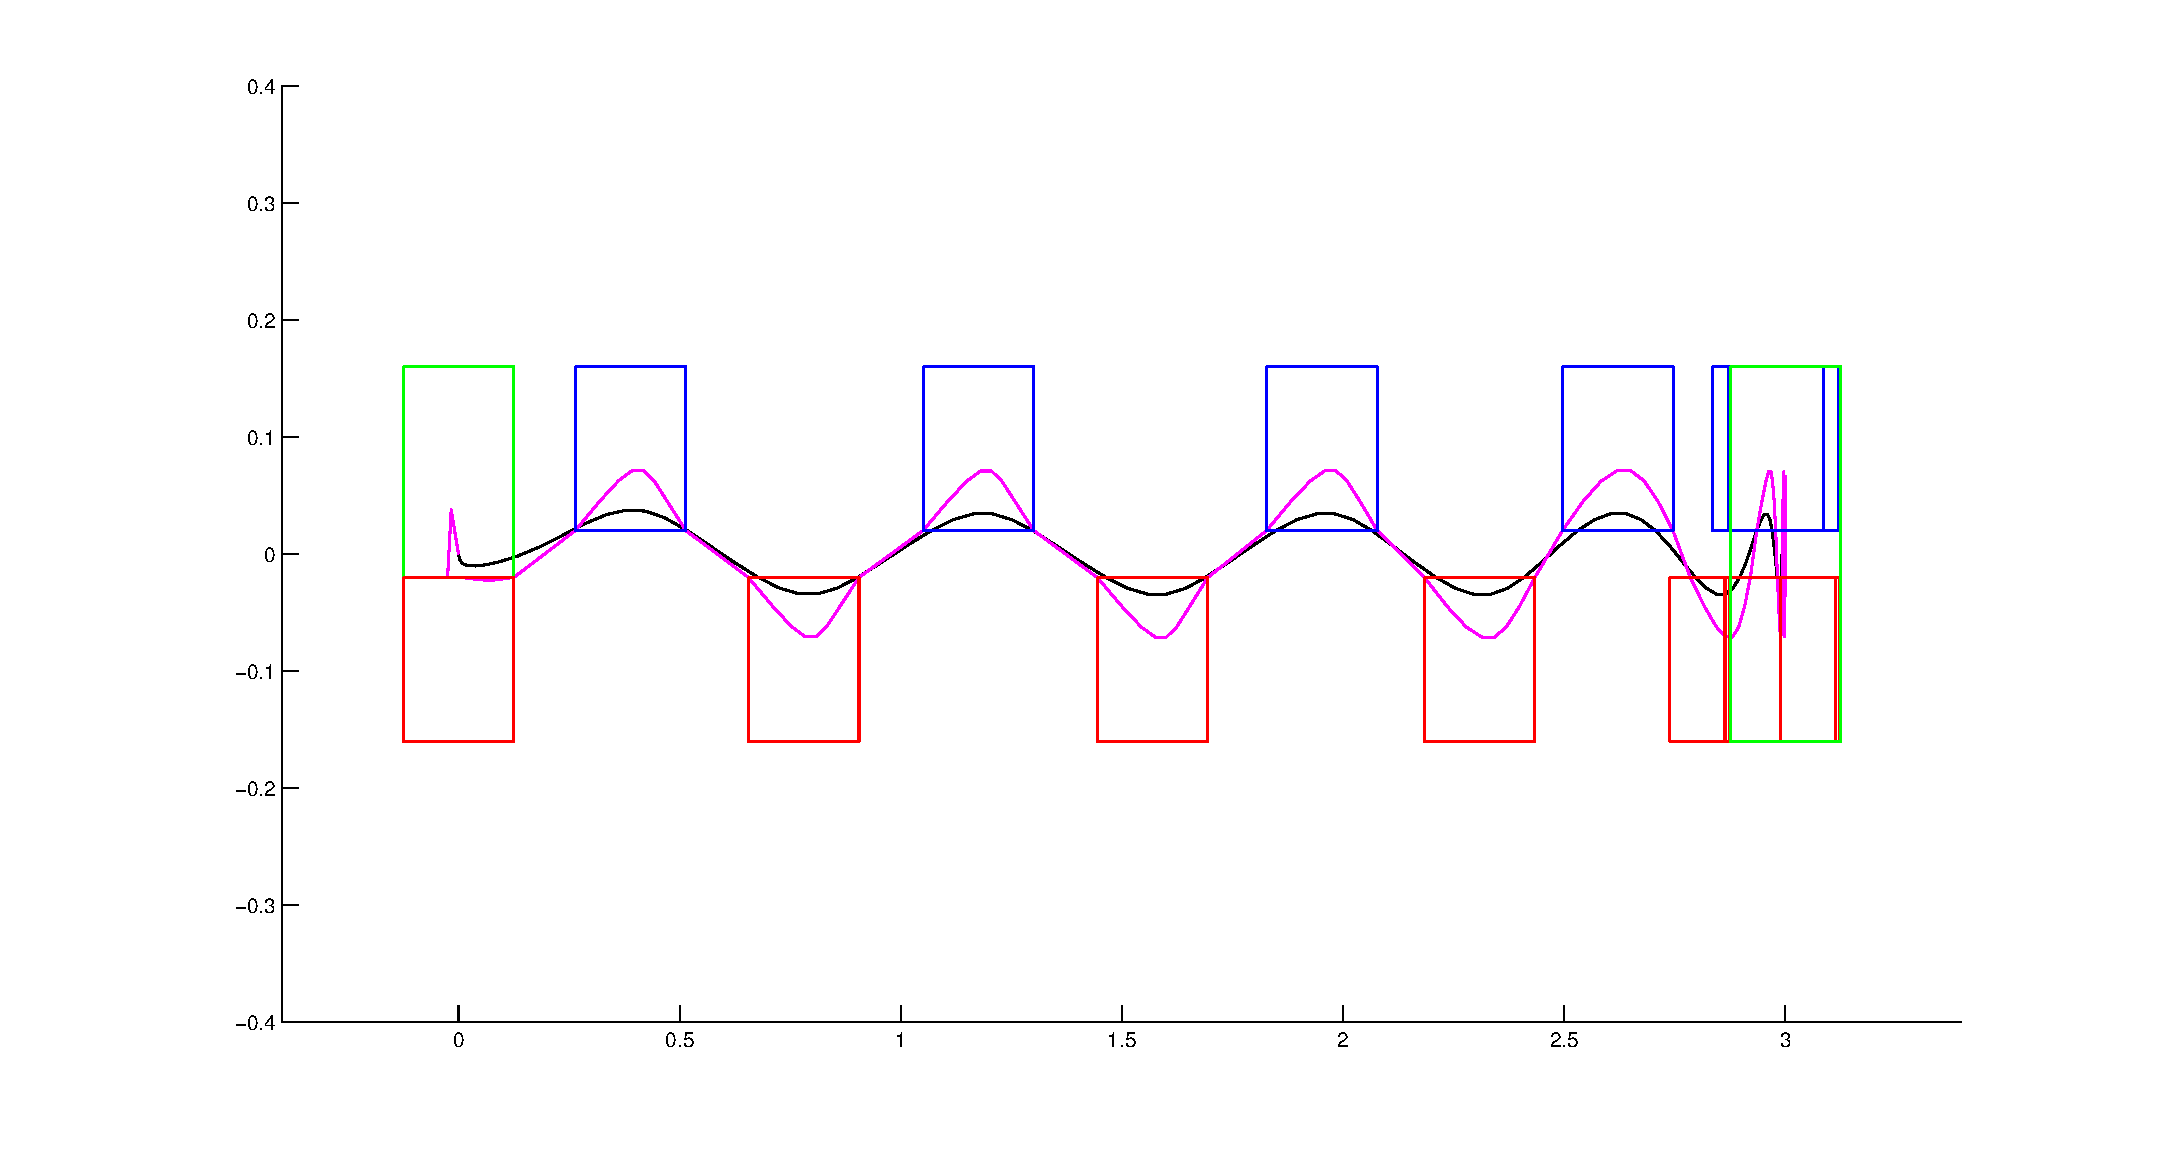
\includegraphics[scale=.18]{Chap4-Visual-Servoing/footsteps_mpc}} ~
 \subfigure{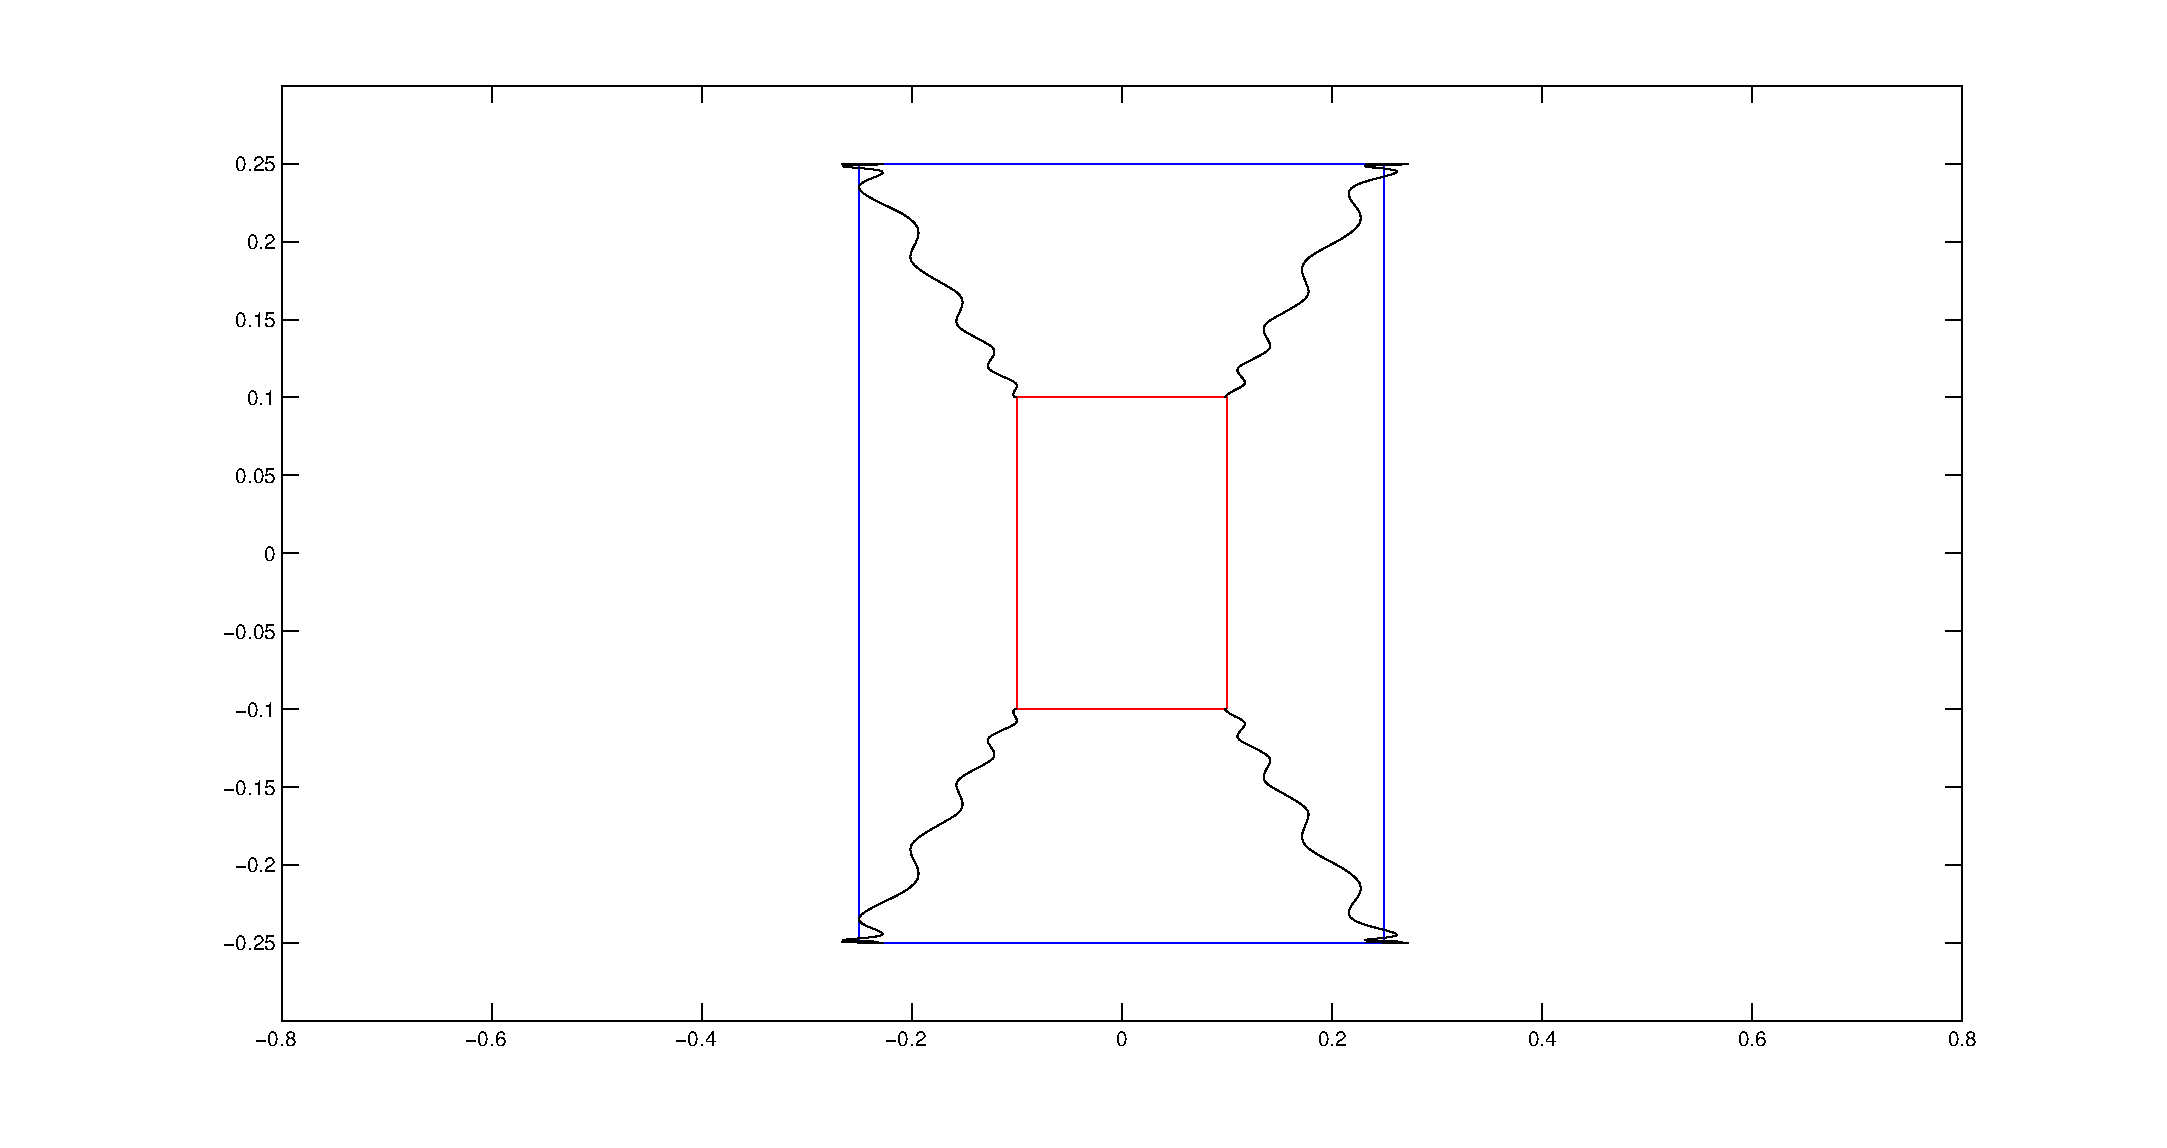
\includegraphics[scale=.18]{Chap4-Visual-Servoing/features_mpc}} \\
 \subfigure{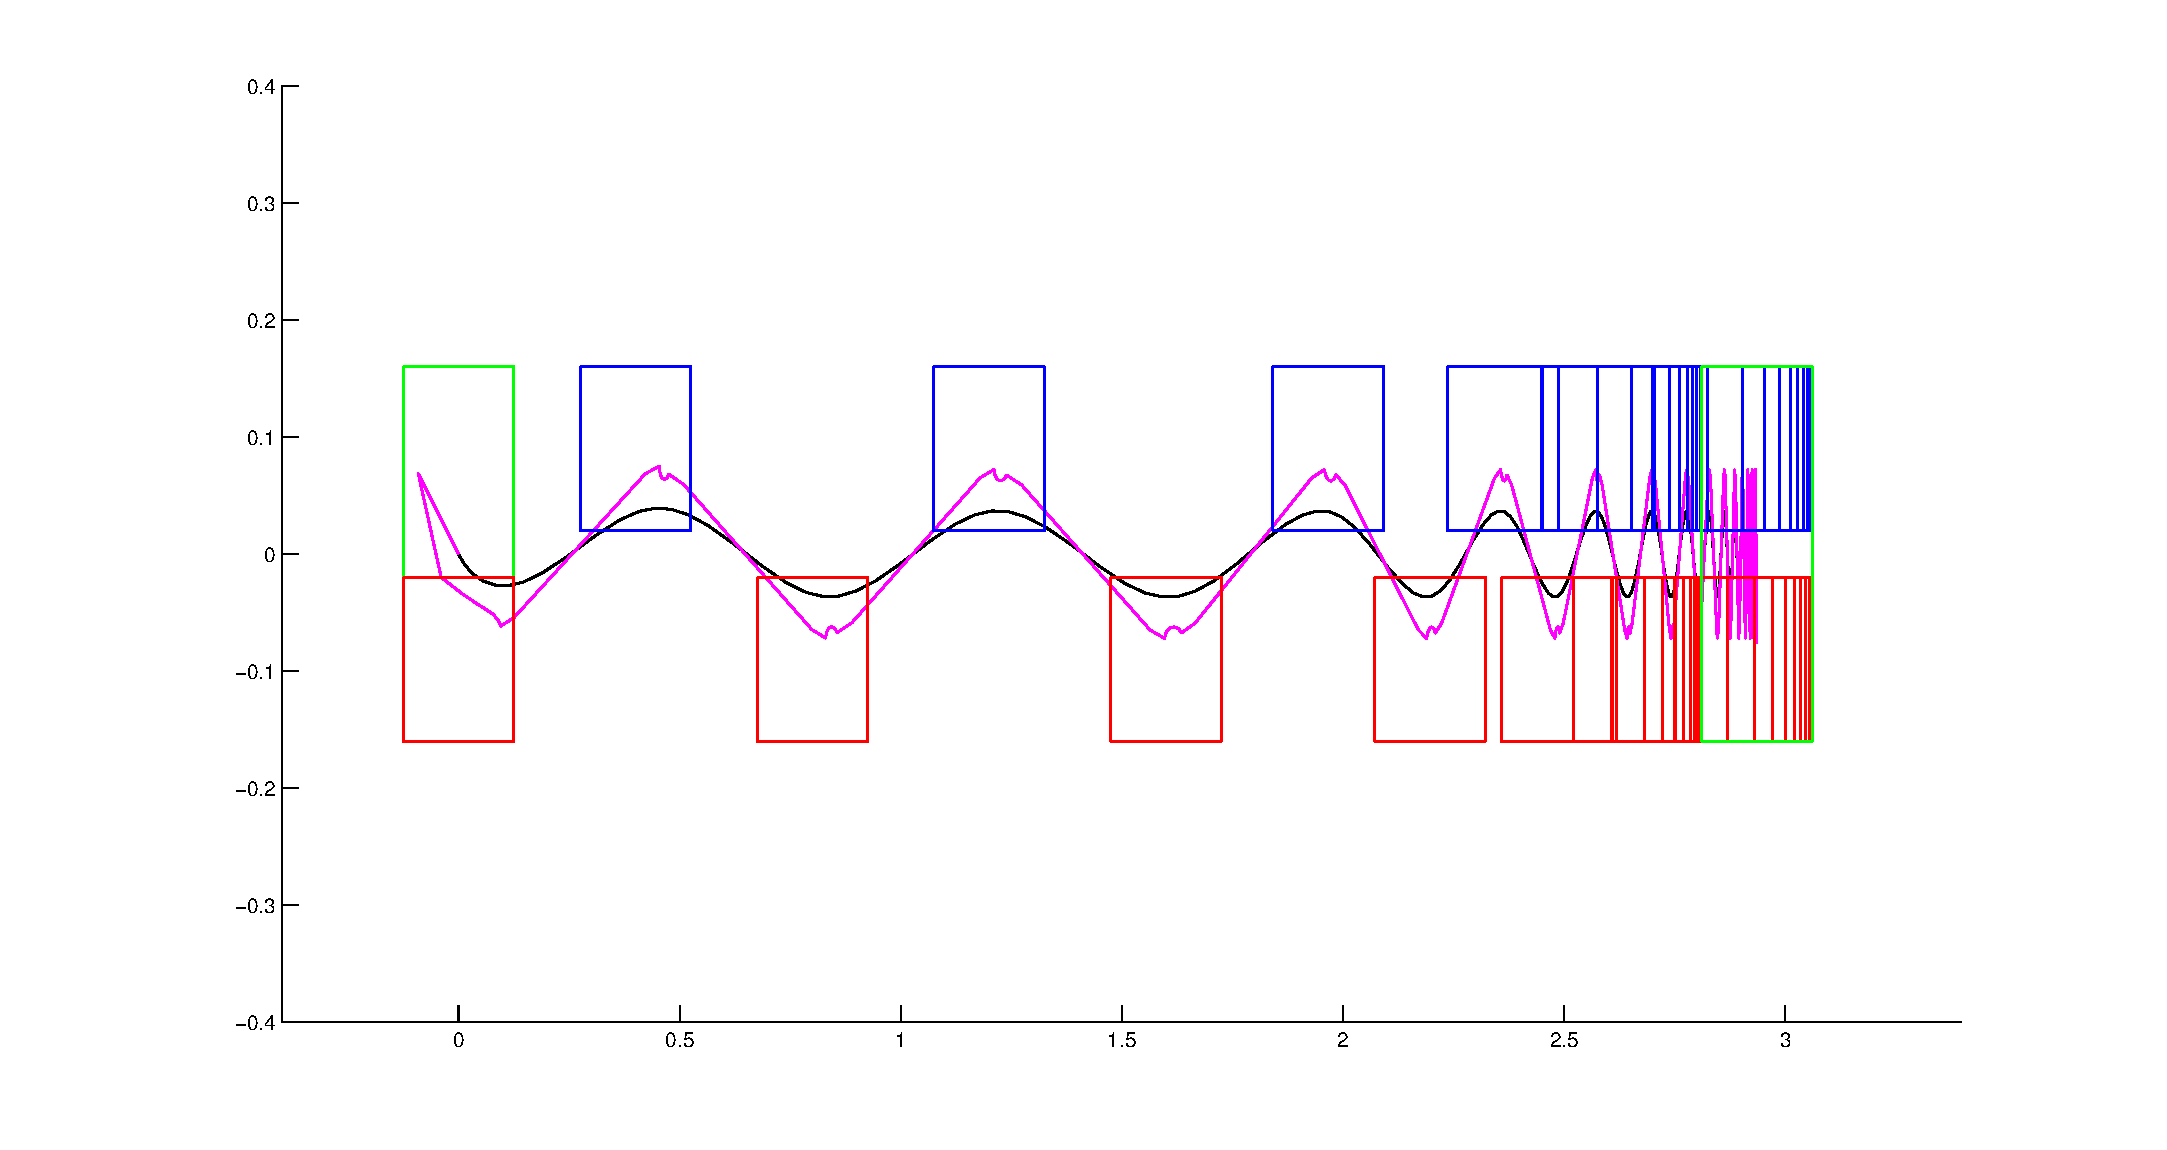
\includegraphics[scale=.18]{Chap4-Visual-Servoing/footsteps_classical-vs}} ~
 \subfigure{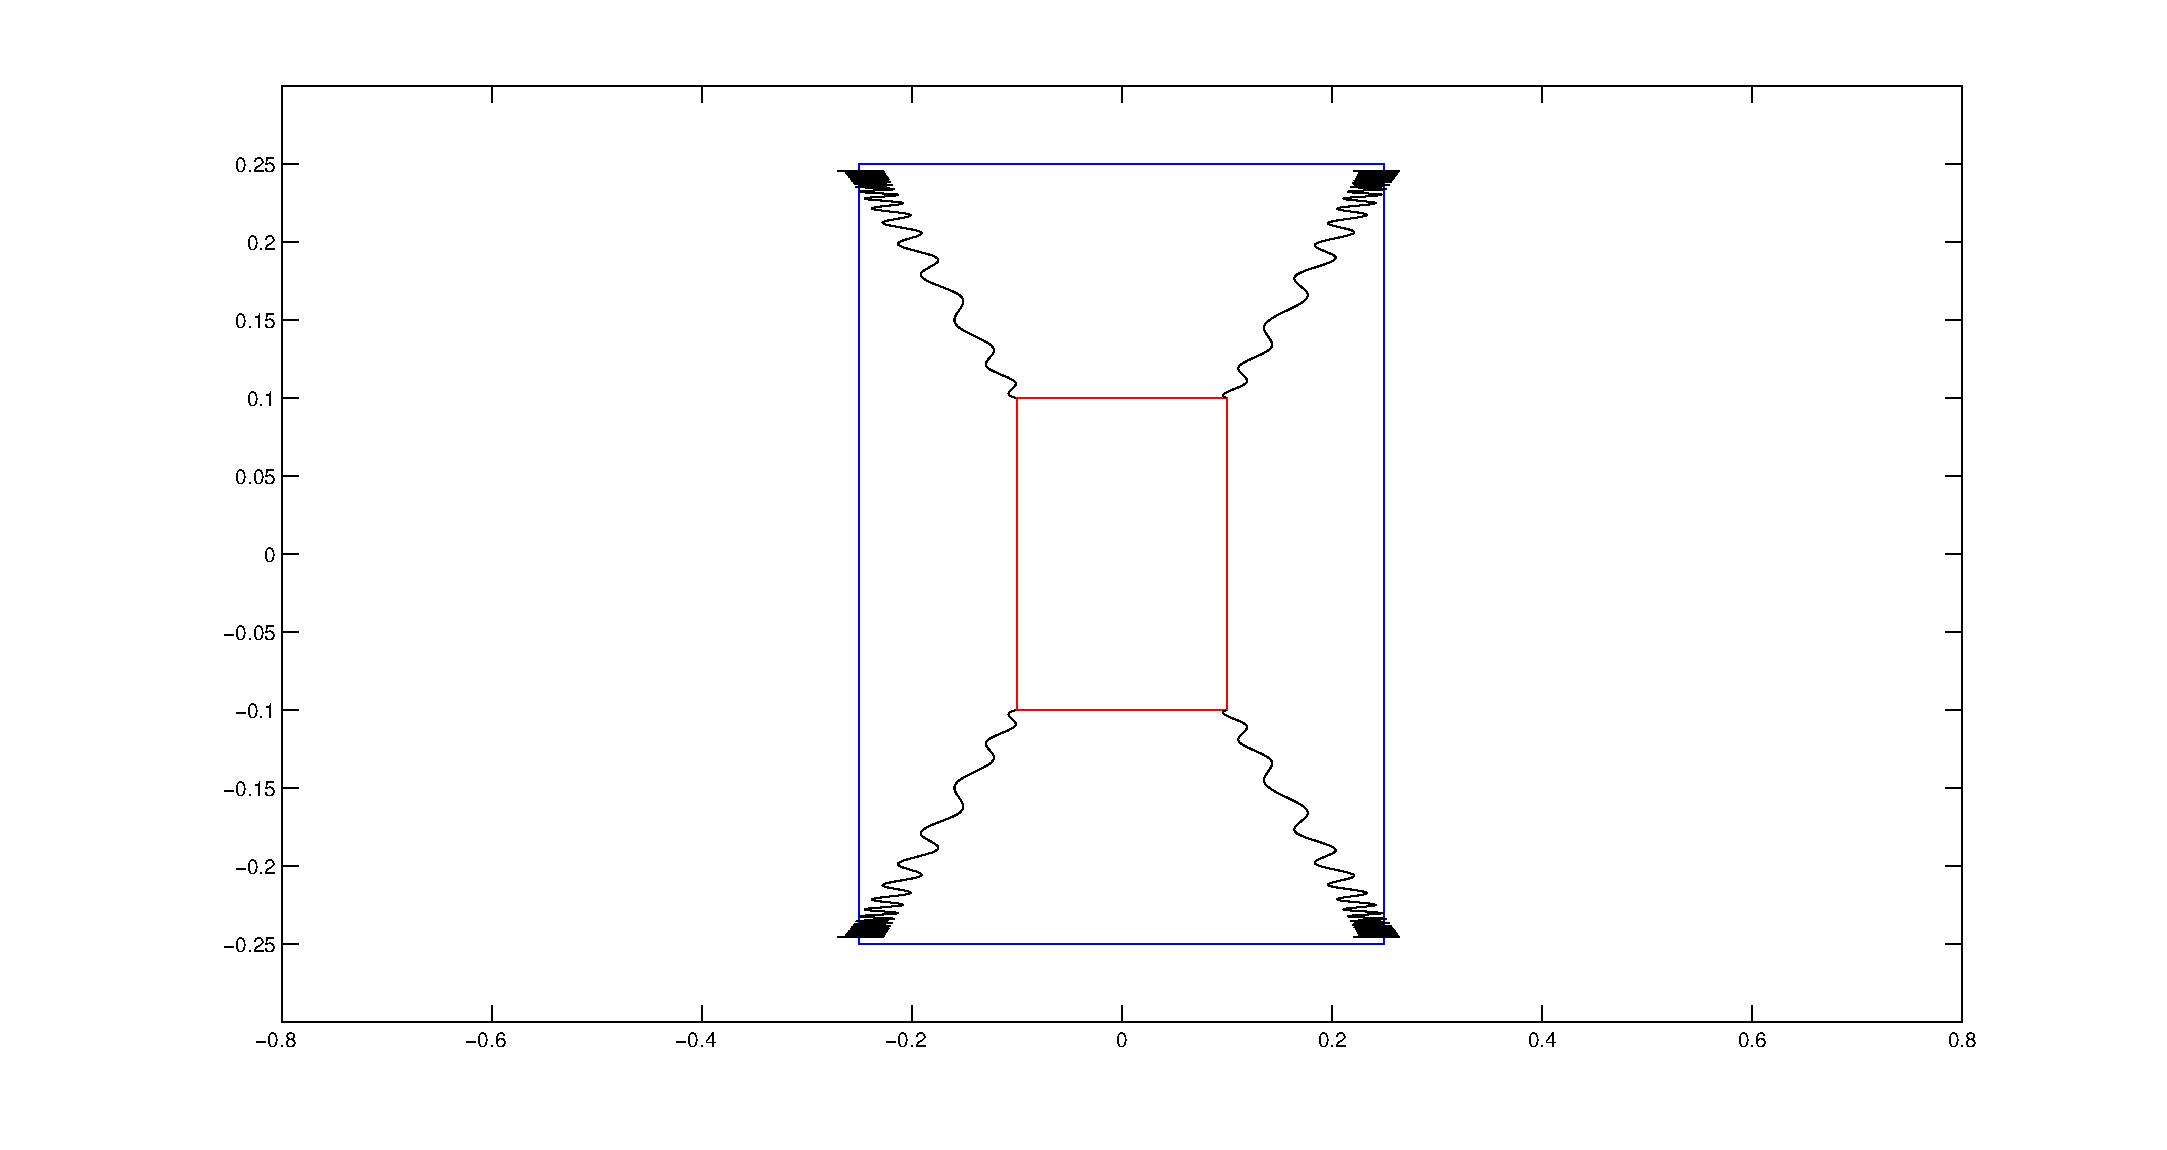
\includegraphics[scale=.18]{Chap4-Visual-Servoing/features_classical-vs}}
 \caption{\label{Fig:Comparisons-approaches} Comparison between the coupled (up) and decoupled approaches (bottom). On the left side, we depict the robot trajectory with the footsteps (red and blue), and the CoM (black) and CoP (pink) trajectories. On the right side, we depict the evolution of the instantaneous features positions during the experiment (from the red rectangle, at the beginning of the simulation, to the blue one, at the end).}
 \end{figure*}

\begin{figure*}[ht]
 \centering
 \subfigure{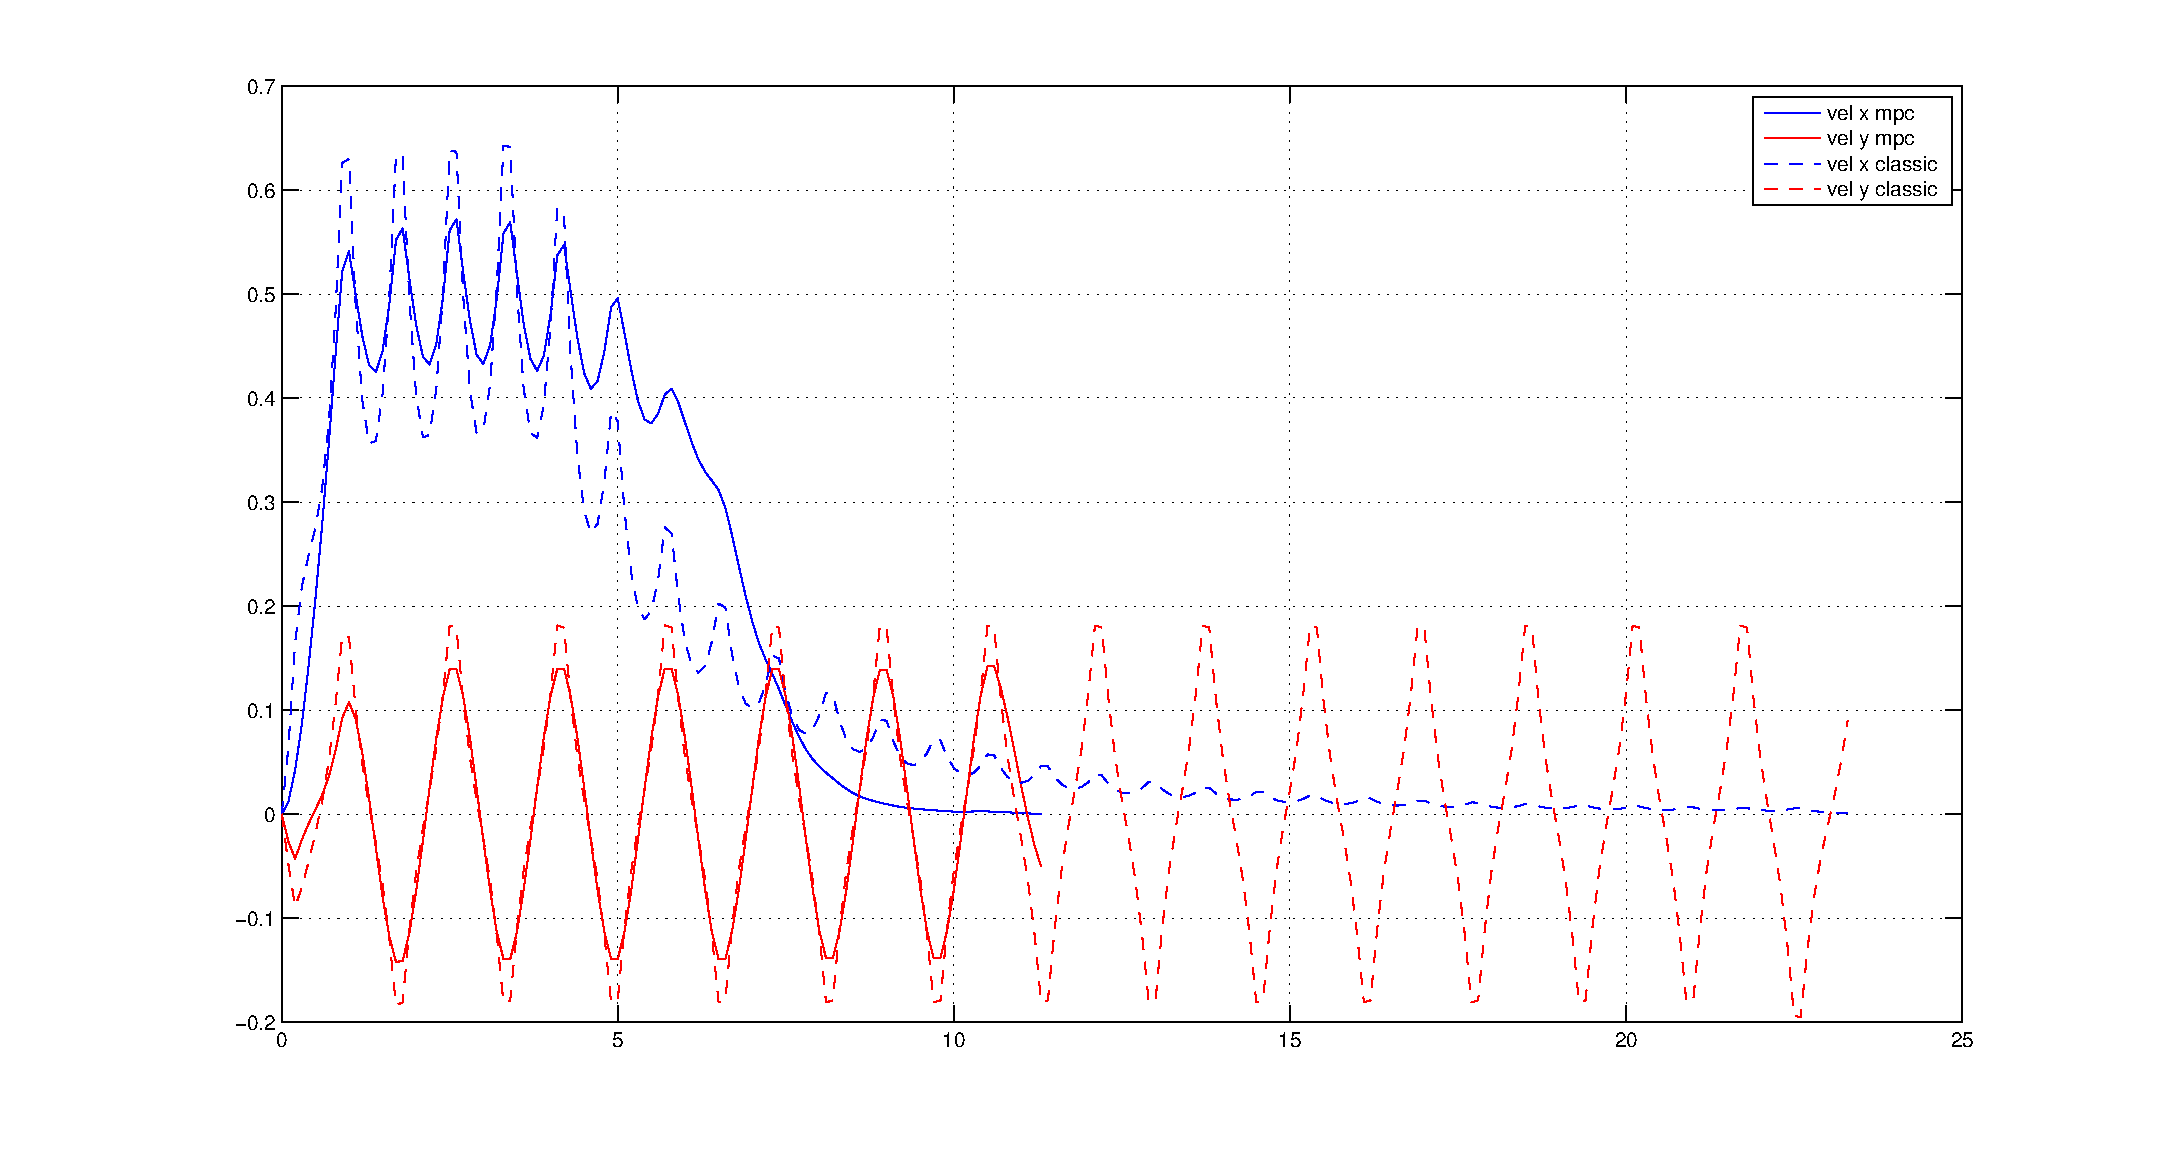
\includegraphics[scale=.3]{Chap4-Visual-Servoing/velocities_both}}
 \subfigure{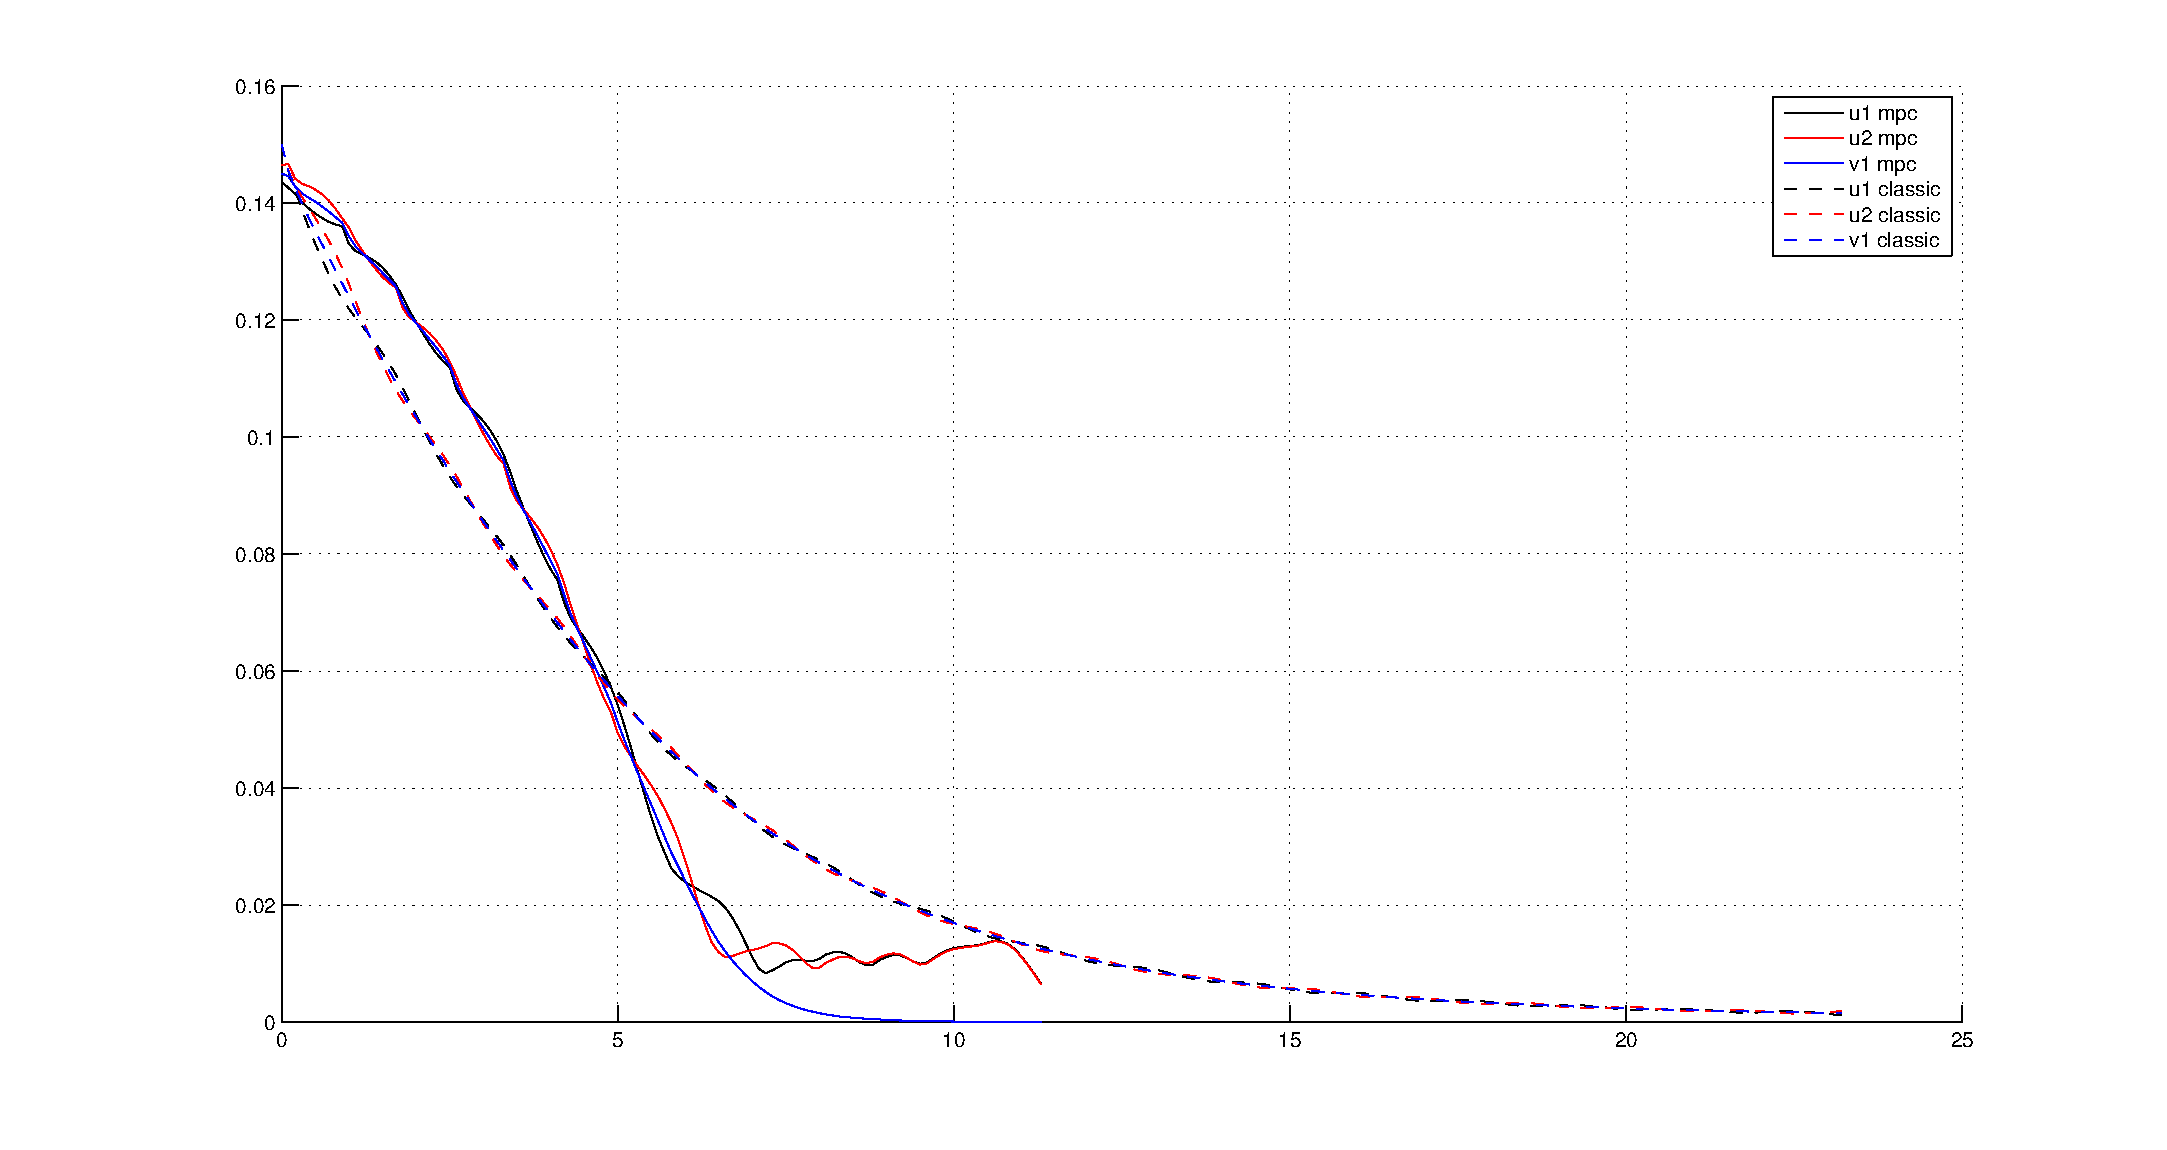
\includegraphics[scale=.3]{Chap4-Visual-Servoing/errors_both}}
 \caption{\label{Fig:Comparisons-velocitieserrors} Left, comparison of velocity profiles in the $x$ (blue) and $y$ (red) axis, for the decoupled (dashed line) and coupled (solid line) approaches. Right, comparison of the features errors evolution.}
 \end{figure*}

We conducted a simple experiment to illustrate better the differences between the two approaches of Section~\ref{sec:vsclaire} and Section~\ref{sec:vsmauricio}, and to have quantitative comparisons between them. In this experiment, the robot has simply to go three meters forward. In Fig.~\ref{Fig:Comparisons-approaches}, we depict the robot trajectories and footsteps (left column) and the features trajectories (right column) for each approach (the coupled one in the upper line, the decoupled one in the lower line). We can clearly appreciate that the coupled approach converges faster. Indeed, with the coupled approach, it took 15 steps (including double supports) to reach the goal. However, with the decoupled approach, after 30 steps, the goal  has still not been reached and keeps converging slowly. Here, the convergence criterion is the norm of the errors between the current features positions and the desired ones. Moreover, one can observe that, close to the goal, the features positions follow a smoother trajectory in the case of the visual predictive control than with the decoupled approach, where oscillations (as a result of the immediate stepping) are visible.

In Fig.~\ref{Fig:Comparisons-velocitieserrors} left, we present the profiles of velocities performed by the robot, in both cases. It is interesting to note that in the coupled approach, the amplitude of the oscillations is smaller, which is desirable. Also, when the error gets small, the classical approach slows down to have a slow convergence rate. This is a normal feature of classical visual servoing, i.e. the error evolves with an exponential decay. In the decoupled approach, this behavior is clearly present. However, in the coupled approach combining the MPC walking pattern generator with visual predictive control, this is not true anymore, see Fig.~\ref{Fig:Comparisons-velocitieserrors} right, in particular, because we take into account future information, so the coupled system converges faster. In the errors evolution, we use the same symmetry argument as in Fig.~\ref{Fig:Results6}. We should note that the $u$ components in the image plane are theoretically the oscillatory ones (from the stepping motion). In Fig.~\ref{Fig:Comparisons-velocitieserrors}, we can see that the $v$ component converges faster in the coupled approach. With the $u$ components, there remains a small residual of the oscillation in both the coupled and decoupled approaches, which explains that the $u$ components converge slower in the coupled approach.


\section{Conclusion}
\label{sec:conclusions}
Since the original proposal for walking generation proposed in~\citep{Kajita2003}, most of the efforts in the literature have focused in dynamical balance and stability. In this chapter, we have proposed a novel approach to close the control loop by introducing visual information into the walking pattern generation. Our online pattern generator integrates the regulation of the relative pose of image features while simultaneous ensuring safety and stability. In order to keep the optimization formulation as a QP, the perspective projection equations have been linearized around the features positions at the beginning of each cycle. However, our current approach uses 3D information that strongly depends on the localization. As an ongoing work, we wish to drop the need of 3D information by predicting the image positions of the landmarks in terms on the velocity of the robot in the horizon (IBVS); we also plan to perform real experiments on the HRP-2 humanoid platform.
